\documentclass[11pt,a4paper,twoside,pdf]{article}

% Paquetes (añade otros si los necesitas):
\usepackage{latexsym}
\usepackage[utf8x]{inputenc}
\usepackage{soul}
\usepackage{array}
\usepackage{amsmath}
\usepackage{amssymb}
\usepackage{marvosym}
\usepackage{epsfig}
\usepackage{graphics}
\usepackage{amsfonts}
\usepackage{xspace}
\usepackage{color}
\usepackage{booktabs}
\usepackage{xtab}
\usepackage[colorlinks=true,urlcolor=blue,linkcolor=blue,citecolor=blue]{hyperref}
\numberwithin{equation}{section}

% Paquetes extra
\usepackage{listings}

% Fuente: palatino
\usepackage[sc]{mathpazo}
\linespread{1.05}

% TFG en inglés:
%\usepackage[english]{babel} 
%\addto\captionsenglish{\renewcommand{\chaptername}{}}

% TFG en español:
\usepackage[spanish,es-nodecimaldot,es-tabla,es-lcroman,es-nosectiondot,
            es-noindentfirst]{babel}
\renewcommand\spanishchaptername{}

% Formato de la página:
\usepackage{fancyhdr}
\usepackage[top=2.88cm,bottom=2.97cm,left=2.95cm,right=2.95cm]{geometry}
\setlength{\parskip}{0.1cm}

% Pon aquí tus definiciones:

\newcommand{\dis}{\displaystyle}
\sodef\an{}{.2em}{1em plus1em}{2em plus.1em minus.1em}

\begin{document}

% Índice  %%%%%%%%%%%%%%%%%%%%%%%%%%%%%%%%%%%%%%%%%%%%%%%%%%%%%%%%%%%%%%%%%%%%%%

% Portada %%%%%%%%%%%%%%%%%%%%%%%%%%%%%%%%%%%%%%%%%%%%%%%%%%%%%%%%%%%%%%%%%%%%%%

\pagestyle{empty}


\noindent
\begin{tabular}{r}

\includegraphics[width=8.8cm]{escudoUGRmonocromo.png} \\[-1.8ex]
\hspace{31mm}\vspace{-8mm}
\begin{tabular}{c}
\hline\\[-1ex]\hskip-2mm
{\bf Facultad de Ciencias}\hspace{18mm}
\end{tabular}
\end{tabular}

{\large
\vspace{30mm}
\hspace{25mm}
\begin{tabular}{l}
\an{GRADO EN F\'ISICA}
\end{tabular}

\vspace{45mm}
\hspace{25mm}
\begin{tabular}{l}
\an{APUNTES B\'ASICOS}
\\[1.5ex]
\an{\LARGE\bf GNUPLOT PARA F\'ISICOS}
\end{tabular}

\vfill
\hspace{25mm}
\begin{tabular}{l}
Presentado por:
\\
{\bf D. David Ortiz del Campo}
\\[3ex]
Curso Académico 2019/2020
\end{tabular}
}


\newpage
\clearpage
\vspace*{\fill}

\begin{center}

{\bf Resumen}
\bigskip

\begin{minipage}{0.8\linewidth}
En este texto se hará una introducción a gnuplot como herramienta para procesar datos y graficarlos, así como algunos trucos para poder mejorar la apariencia de nuestras gráficas y la eficiencia al usar gnuplot. De todas formas, es siempre aconsejable complementar lo aquí dicho con lo que se pueda encontrar en otras fuentes y con la experiencia al usarlo.
\end{minipage}




\end{center}

\vfill \clearpage

% Indice %%%%%%%%%%%%%%%%%%%%%%%%%%%%%%%%%%%%%%%%%%%%%%%%%%%%%%%%%%%%%%%%%%%%%%%
\newpage

\tableofcontents

% Texto %%%%%%%%%%%%%%%%%%%%%%%%%%%%%%%%%%%%%%%%%%%%%%%%%%%%%%%%%%%%%%%%%%%%%%%%
\newpage

\pagestyle{fancy}
\fancyhead[RO,LE]{\leftmark}
\fancyhead[LO,RE]{\thepage}
\fancyfoot{}

\section{Introducción}

Antes de empezar a aprender el manejo de gnuplot conviene saber primero qué es gnuplot.

\subsection{¿Qué es gnuplot y por qué gnuplot?}

Gnuplot es una herramienta de graficado que funciona en base a comandos. Esto implica que gnuplot no tiene en sí una interfaz gráfica, todo funciona gracias a una serie de comandos que se introducen en una consola o que se escriben en un documento de texto. \\

Respecto a la pregunta del motivo por el que gnuplot es una buena opción hay que decir que:

\begin{itemize}
    \item \textbf{Versatilidad:} Gnuplot tiene un amplio abanico de herramientas que permiten analizar datos, ajustarlos y graficarlos en 2D y en 3D de varias formas distintas.
    \item \textbf{Disponibilidad:} Gnuplot es un proyecto disponible en la amplia mayoría de las plataformas (Linux, OSX, Windows...). Además aunque su código fuente tiene copyright la descarga es completamente gratuita.\cite{gnuplot-5.4-doc}
    \item \textbf{Sencillez y eficiencia:} Es un programa muy sencillo pero que permite una gran eficiencia una vez que se aprende a manejar correctamente.
\end{itemize}

Por todo ello gnuplot es una muy buena alternativa para el graficado de nuestros datos. Además aprendiendo algunos trucos para mejorar la apariencia se pueden conseguir buenos resultados.

\subsection{Instalación}

El procedimiento para instalar gnuplot depende del sistema operativo que estemos utilizando pero en la amplia mayoría de los casos se podrán encontrar en los repositorios del sistema operativo en cuestión. De todas formas podemos encontrar las distintas formas de descargarlo y los archivos necesarios en: \url{http://www.gnuplot.info/download.html}. En caso de realizar la instalación en Windows y estar familiarizado con el uso de CMD es muy aconsejable que se introduzca gnuplot en el PATH. \\

Una vez haya terminado la instalación ejecutamos gnuplot y tiene que salir algo como lo que se muestra en la figura \ref{fig:AbrirGnuplot}. En ella veremos una serie de información sobre gnuplot en sí y sobre la versión que estamos utilizando. Es también útil e interesante ver lo que pone en la penúltima línea: \textit{Terminal type is now...}. Esto nos indica que tipo de terminal estamos usando por defecto, lo cual nos será de ayuda más adelante. Por último, en la última línea vemos que pone \textit{gnuplot} y que se ha quedado el cursor ahí. Es en esta línea donde escribiremos los comandos que queramos utilizar para utilizarlo.

\begin{figure}
    \centering
    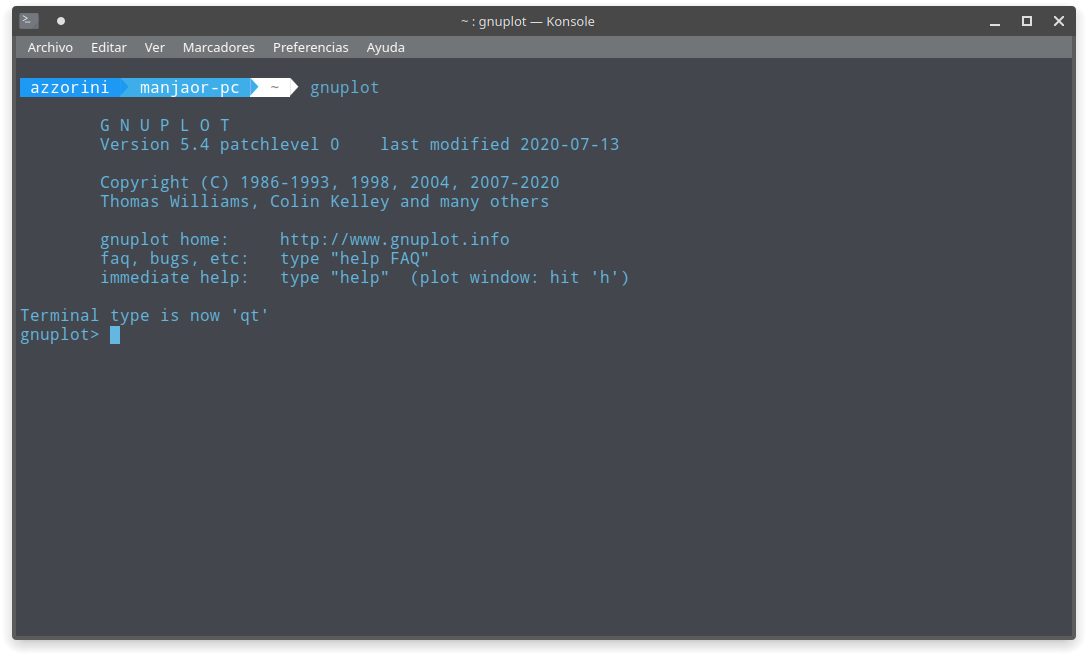
\includegraphics[scale=0.52]{Capturas/00_AbrirGnuplot.png}
    \caption{Texto que nos muestra gnuplot al abrirlo.}
    \label{fig:AbrirGnuplot}
\end{figure}
\newpage

\section{Primeros pasos}

Lo primero de todo que podemos hacer es empezar a trastear gnuplot para ver su uso básico. Sobre la consola que se nos ha abierto similar a la de la imagen \ref{fig:AbrirGnuplot} vamos a escribir el siguiente comando y a pulsar intro.

\begin{lstlisting}[language=Gnuplot]
gnuplot> plot x
\end{lstlisting}

Si se ha realizado todo bien se ha de abrir una ventana como la mostrada en la figura \ref{fig:plot_x_without}. Todavía está muy lejos de ser bonito visualmente pero ya hemos podido conseguir mostrar nuestra primera función.

\begin{figure}[!h]
    \centering
    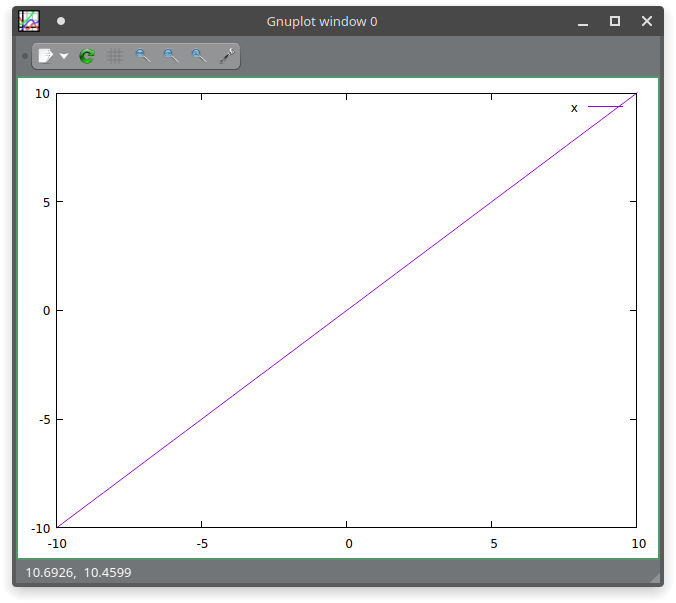
\includegraphics[scale=0.4]{Capturas/01_PrimerPlot.png}
    \caption{Graficado de la función $f(x) = x$ sin ningún formato.}
    \label{fig:plot_x_without}
\end{figure}

% Funciones matemáticas

\subsection{Funciones matemáticas}

Como buen programa destinado al uso científico gnuplot tiene incorporado un gran abanico de funciones matemáticas destinadas a que se puedan mostrar todas las cosas que queramos. Además también se pueden definir nuestras propias funciones y nuestras propias constantes. \\

Como ya se ha mencionado hay un gran número de funciones matemáticas disponibles en gnuplot que se pueden consultar en \url{http://gnuplot.sourceforge.net/docs_4.2/node53.html}. De todas formas vamos a probar algunas de ellas para que sirva de demostración. \\

En primer lugar podemos usar los operadores matemáticos clásicos: $+$, $-$, $*$ y $/$\footnote{Si la división se realiza entre dos números enteros el resultado será otro número entero.}. Además también se puede usar $**$ para elevar un número a otro y $\%$ para sacar el módulo de la división entera. Así por ejemplo si queremos mostrar un polinomio podemos introducir el siguiente comando:

\begin{lstlisting}[language=Gnuplot]
gnuplot> plot 3*x**3 - 4*x**2 + x - 5
\end{lstlisting}

También es posible utilizar una gran variedad de funciones matemáticas de gran interés como pueden ser: el valor absoluto $\text{abs}(x)$, la raíz cuadrada $\text{sqrt}(x)$, la exponencial $\text{exp}(x)$, el seno $\sin(x)$, el coseno $\cos(x)$ y la tangente $\tan(x)$ (así como sus inversas: $\text{asin}(x)$, $\text{acos}(x)$ y $\text{atan}(x)$)\footnote{De no indicar lo contrario todas las funciones trigonométricas trabajarán con radianes.}. También hay otras funciones más específica como la función $\Gamma$ ($\text{gamma}(x)$) o algunas de las funciones de Bessel ($\text{besj0}(x)$, $\text{besj1}(x)$, $\text{besy0}(x)$, $\text{besy0}(x)$, $\text{besy1}(x)$). Antes de seguir cabe destacar que si se quieren mostrar varias gráficas superpuestas simplemente hay que pasárselas a plot separadas por comas.

\begin{lstlisting}[language=Gnuplot]
gnuplot> plot cos(x), 1-x**2
\end{lstlisting}

Por otro lado, en ocasiones es interesante poder definir nuestras propias funciones, es muy sencillo simplemente tendremos que escribir el nombre de la función y sus variables e igualarlo al valor que queremos que tome como se muestra en el siguiente ejemplo:

\begin{lstlisting}[language=Gnuplot]
gnuplot> factor_relativista(x) = 1/sqrt(1-x**2/3e8**2)
gnuplot> plot 1, factor_relativista(x)
\end{lstlisting}

Para finalizar también es posible usar algunas variables que el propio gnuplot nos define o definir nuestras propias variables. La única variable que gnuplot define en todos los casos es $\text{pi}$, aunque puede haber ciertos casos o bajo ciertas acciones en las que el propio programa nos defina otras. Para asignar una variable no tenemos más que escribir el nombre de nuestra variable seguido de un signo igual y del valor que deseamos que tome. Así por ejemplo sería más bonito modificar el ejemplo anterior de la siguiente manera:

\begin{lstlisting}[language=Gnuplot]
gnuplot> c = 3e8
gnuplot> factor_relativista(x) = 1/sqrt(1-(x/c)**2)
gnuplot> plot 1, factor_relativista(x)
\end{lstlisting}

Como se puede observar el resultado es mucho más bonito y mucho más fácil de leer. Además en caso de tener que escribir ese valor varias veces es mucho más cómodo tenerlo asignado en una variable.

\subsection{Límites de graficado}

En muchas ocasiones es de gran interés establecer la región que nos interesa de la gráfica que vamos a mostrar. De hecho, si habéis probado alguno de los ejemplos anteriores os habréis dado cuenta de que los límites que aparecen son los que muestra gnuplot por defecto y no son de gran utilidad en muchas de las gráficas. \\

Para redefinir estos límites tenemos que hacer uso de un comando que de aquí en adelante usaremos mucho: $\text{set}$. En este caso tenemos que decir que queremos cambiar el rango a mostrar en el eje $x$ y en el eje $y$. Por lo tanto los comandos a escribir son $\text{set xrange}$ y $\text{set yrange}$. Aunque si no queremos escribir mucho podemos usar $\text{set xr}$ y $\text{set yr}$. Después de esto tenemos que especificar el rango en el formato [límite inferior:límite superior]. Así por ejemplo podemos cambiar el rango de algún ejemplo anterior:

Ejemplo del coseno comparado con $1-x^2$:

\begin{lstlisting}[language=Gnuplot]
gnuplot> set xrange [0:pi]
gnuplot> set yrange [-1:1]
gnuplot> plot cos(x), 1-x**2
\end{lstlisting}

Ejemplo del factor relativista:

\begin{lstlisting}[language=Gnuplot]
gnuplot> c = 3e8
gnuplot> set xr [0:c]
gnuplot> set yr [0:7]
gnuplot> factor_relativista(x) = 1/sqrt(1-(x/c)**2)
gnuplot> plot 1, factor_relativista(x)
\end{lstlisting}

\subsection{Crear y ejecutar un script}

Una de las grandes comodidades de gnuplot es el poder crear scripts que ejecuten una tarea concreta. Esto facilita trabajar cuando necesitamos insertar muchos comandos y, por otro lado, nos permite reutilizar los scripts en distintas ocasiones. \\

Los scripts no son más que ficheros de texto en los que iremos metiendo línea a línea cada comando de los que queremos ejecutar. No obstante hay que añadir una cosa que hasta ahora no hemos añadido. Veamos primero un ejemplo y ahora lo explicaremos:

\begin{lstlisting}[language=Gnuplot]
set terminal png
set output "grafica.png"
\end{lstlisting}

Analicemos los comandos línea a línea. La primera línea ajusta el tipo de terminal, esto sirve para especificar cual es el tipo de archivo en el que queremos que la gráfica salga. De momento lo vamos a dejar como una imagen PNG pero existen muchas más opciones que hablaremos en el apartado \ref{subsec:TiposTerminales}. \\

En la segunda línea podemos ver que se configura el archivo en el que queremos que nos guarde la gráfica. Si no se especifica nada se guardará en la misma carpeta en la que estemos ejecutando gnuplot (en caso de duda se puede escribir pwd para ver en qué directorio estamos y podemos cambiar de directorio usando cd ``[NOMBRE DIRECTORIO]''). También es posible indicar una ruta en la que podemos guardar el archivo por ejemplo: ``C:\textbackslash\textbackslash Users\textbackslash\textbackslash Miuser\textbackslash\textbackslash Desktop\textbackslash\textbackslash grafica.png'' en Windows y ``/home/miuser/Escritorio/grafica.png'' en Linux. \\

De esta forma por ejemplo podemos escribir el siguiente script para el ejemplo del factor relativista:

\begin{lstlisting}[language=Gnuplot]
set terminal png
set output "relatividad.png"
c = 3e8
set xr [0:c]
set yr [0:7]
factor_relativista(x) = 1/sqrt(1-(x/c)**2)
plot 1, factor_relativista(x)
\end{lstlisting}

Una vez que tenemos el script creado y guardado en una carpeta tenemos dos opciones para ejecutarlo:

\textbf{Opción 1}: Esta es la opción ``externa'' y para ello es necesario tener gnuplot en el PATH (hay que configurarlo en el caso de Windows). Abriremos una consola en el directorio donde tenemos el script y escribiremos: gnuplot [nombre de script]. También es posible poner la ruta para ejecutarlo desde otro directorio. \\

\textbf{Opción 2}: Esta es la opción ``interna''. Para ello abriremos gnuplot y nos iremos (usando cd o abriendo directamente donde esté el script) al directorio donde tenemos el script. Tamnbién es posible ahorrarse esto si luego se especifica la ruta al archivo. Ahora ejecutaremos la orden:

\begin{lstlisting}[language=Gnuplot]
gnuplot> load "NombreScript.plt"
\end{lstlisting}

Con todo esto ya es posible crear y ejecutar nuestros propios scripts. A partir de ahora se utilizarán scripts en la mayoría de los ejemplos entendiendo que ya se saben utilizar.

\section{Manejo general}

\subsection{Configuración del título y de los labels}

En muchas ocasiones es de gran interés modificar el título de la gráfica y los labels de cada eje para indicar de qué trata la gráfica así como lo que se ha representado en cada eje y sus unidades. \\

Para configurar el título usaremos: set title ``Información que queremos que salga en el título''. Así mismo para cambiar los labels pondremos: set xlabel ``Información del xlabel'' y set ylabel ``Información del ylabel''. Es posible también abreviar y en lugar de xlabel e ylabel poner xl e yl respectivamente. De esta forma podemos reescribir el script del factor relativista para que muestre esta información:

\begin{lstlisting}[language=Gnuplot]
set terminal png
set output "relatividad.png"

set title "Relatividad galileana frente a relatividad especial"
set xlabel "Velocidad relativa [m/s]"
set ylabel "Dilatacion temporal [s]"
c = 3e8
set xr [0:c]
set yr [0:7]
factor_relativista(x) = 1/sqrt(1-(x/c)**2)
plot 1, factor_relativista(x)
\end{lstlisting}

\subsection{Palabras a mostrar en la leyenda}

Como habréis visto hasta el momento nos aparecen en la parte superior derecha de la gráfica información sobre las distintas cosas que se han mostrado en la gráfica. No obstante, aparecen directamente las funciones que hemos mostrado y es más útil poner un texto a nuestra elección. Para ello tenemos que modificar la línea en la que usamos plot añadiendo después de cada función la palabra ``title'' (o su abreviatura ``t'') junto con la información que se quiere poner entre comillas:

\begin{lstlisting}[language=Gnuplot]
plot f(x) title "Primera", g(x) title "Segunda"
\end{lstlisting}

Así por ejemplo podemos modificar el script del factor relativista para añadir títulos a las funciones a graficar:

\begin{lstlisting}[language=Gnuplot]
set terminal png
set output "relatividad.png"

set title "Relatividad galileana frente a relatividad especial"
set xlabel "Velocidad relativa [m/s]"
set ylabel "Dilatacion temporal [s]"
c = 3e8
set xr [0:c]
set yr [0:7]
factor_relativista(x) = 1/sqrt(1-(x/c)**2)
plot 1 t "R. Galileana", factor_relativista(x) t "R. Especial"
\end{lstlisting}

En caso de que no se quiera mostrar nada en la leyenda para una gráfica en concreto se tiene que poner la palabra title seguida de dos comillas sin nada entre ellas: plot h(x) t ``''.

\subsection{Ajustar la leyenda}

Ahora que sabemos como modificar el texto a mostrar en la leyenda es una buena oportunidad para aprender los ajustes que se le pueden hacer. Así como si se quiere mostrar o no. Para ver la totalidad de las opciones que existen se puede ejecutar: help set key. No obstante aquí veremos algunas de las cosas más importantes.

\textbf{1. No mostrar la leyenda:} En algunas ocasiones quizás prefiramos no mostrar la leyenda. Para ello tenemos dos opciones la primera de ellas es usando el comando unset:

\begin{lstlisting}[language=Gnuplot]
unset key
\end{lstlisting}

Aunque resulte un poco irónico también es posible quitar la leyenda con el comando set de la siguiente manera:

\begin{lstlisting}[language=Gnuplot]
set key off
\end{lstlisting}

\textbf{2. Leyenda dentro de la gráfica o fuera de la gráfica:} Por defecto la leyenda en gnuplot se coloca dentro de la gráfica pero en algunas ocasiones esto puede hacer que no se vea la gráfica claramente para ello después de poner ``set key'' hay que añadir la opción ``outside''. En caso de querer volver a poner la leyenda dentro solo hay que volver a ejecutarlo con la opción ``inside''.

\begin{lstlisting}[language=Gnuplot]
set key outside
\end{lstlisting}

\textbf{3. Posición de la leyenda:} Independientemente de donde esté la leyenda (dentro o fuera) podremos usar [top, center o bottom] + [left, center o right] para indicar la posición donde queremos que salga la gráfica.\footnote{Nuevamente también es posible abreviar cada una de las palabras de posición y poner solo la primera letra.} Algunos ejemplos podrían ser: ``set key top left'' o ``set key outside bottom center''.\\

\textbf{4. Posición de la leyenda dentro de la gráfica:} Cuando la leyenda está dentro de la gráfica además de lo que ya se ha visto también se puede usar la opción at para indicar unas coordenadas concretas dentro de la gráfica. En concreto se ha de añadir ``at x, y''. Por ejemplo se podría poner:

\begin{lstlisting}[language=Gnuplot]
set key at 2, 8
\end{lstlisting}

\textbf{5. Añadir un título a la leyenda:} También es posible añadirle un título a la leyenda usando la opción ``title''. La sintaxis sería la siguiente:

\begin{lstlisting}[language=Gnuplot]
set key top center title "Leyenda"
\end{lstlisting}

\textbf{6. Poner un recuadro:} También es posible añadir un cuadro a la leyenda usando la opción ``box''.\\

\textbf{7. Configurar el espaciado entre los diferentes elementos de la leyenda:} Para esto utilizaremos la opción ``spacing'' seguido del espaciado que queremos que se aplique. Para hacernos una idea el valor que gnuplot aplica por defecto es $1.25$.\\

También existen otras opciones para configurar el tamaño y estilo de las líneas del recuadro (en caso de ponerlo) que son ``linestyle'', ``linetype'' y ``linewidth'' que pueden ser utilizadas según el apartado \ref{subsec:EstiloLinea}. Por último hay una opción que también puede ser útil que es ``noautotitle''. Esta opción evita que gnuplot genere entradas automáticas a la leyenda cuando no se ha especificado nada y solo acepta aquellas entradas que explícitamente indiquemos.

\subsection{Mostrar datos de un fichero\label{subsec:DatosFichero}}

En muchas ocasiones se querrán mostrar los datos de un fichero con distintos puntos que ya tenemos guardados, en este caso también es posible usar gnuplot para mostrarlos de forma cómoda. Supongamos que tenemos un fichero llamado ``data.dat'' que contiene la información mostrada en la tabla \ref{tab:data_plot_fichero}.

\begin{table}[h]
    \centering
    \caption{Contenido fichero ``data.dat''.}
    \vspace{10pt}
    \label{tab:data_plot_fichero}
    \begin{tabular}{cc}
        \# $x$ & $y$ \\
        \ \ 1 & 1 \\
        \ \ 2 & 2 \\
        \ \ 3 & 3 \\
        \ \ 4 & 4 \\
    \end{tabular}
\end{table}

Cabe destacar que gnuplot no le hará caso a la primera línea puesto que el caracter ``\#'' lo usa gnuplot para indicar comentarios y es una información que el programa obvia pero que puede ser útil para entender el contenido del fichero. Si lo queremos mostrar de forma básica solo tenemos que usar el comando ``plot'' y mandarle el nombre del fichero si estamos en el mismo directorio o su ruta entera de estar en otro directorio. Por ejemplo, podríamos hacer el siguiente script para mostrar el fichero:

\begin{lstlisting}[language=Gnuplot]
set terminal png
set output "data.png"

unset key
set xr [0:5]
set yr [0:5]
plot "data.dat"
\end{lstlisting}

Por defecto se nos muestran una serie de puntos con los datos, no obstante se puede configurar esto para mostrar la gráfica con líneas o con cajas (como si fuera un histograma). Para ello hay que añadir al comando plot la opción ``with lines'' para mostrar líneas o ``with boxes'' para mostrar cajas. \\

También es posible que en ocasiones contemos con ficheros de más de dos columnas en los que queremos mostrar varias funciones distintas. Por ejemplo, supongamos que tenemos el archivo ``data2.dat'' con datos de las funciones $y(x)$ y $z(x)$. Los datos del archivo se muestran en la tabla \ref{tab:data_plot_columnas}. \\

\begin{table}[h]
    \centering
    \caption{Contenido fichero ``data2.dat''.}
    \vspace{10pt}
    \label{tab:data_plot_columnas}
    \begin{tabular}{ccc}
        \# $x$ & $y$ & $z$ \\
        \ \ 1 & 1 & 2 \\
        \ \ 2 & 2 & 4\\
        \ \ 3 & 3 & 6\\
        \ \ 4 & 4 & 8\\
    \end{tabular}
\end{table}

Ahora bien para indicar las columnas que queremos que gnuplot muestre tenemos que utilizar una opción del comando ``plot'' llamada ``using''. La sintaxis es:

\begin{lstlisting}[language=Gnuplot]
plot "fichero.dat" using columna_x:columna_y
\end{lstlisting}

Donde columna\_x es el número de la columna que queremos usar como variable y columna\_y es el número de la columna que queremos usar como los valores de la función. Así pues, si se quieren mostrar las funciones $y(x)$ y $z(x)$ según los datos de la tabla \ref{tab:data_plot_columnas} se puede usar el siguiente script\footnote{En la penúltima línea podemos observar que se ha introducido un ``\textbackslash'' al final de la línea. Esto le indica a gnuplot que la línea (y por lo tanto el comando) no se acaba si no que continua en la siguiente. Es una forma elegante de dividir líneas que se nos hagan muy largas y que usaremos de aquí en adelante.}:

\begin{lstlisting}[language=Gnuplot]
set terminal png
set output "data2.png"

set key top left
set xr [0:5]
set yr [0:10]
plot "data2.dat" using 1:2 t "y(x)",\
    "data2.dat" using 1:3 t "z(x)"
\end{lstlisting}

También es posible escribir un poco menos en nuestros scripts con los dos siguientes atajos. En primer lugar, se puede poner ``u'' en lugar de ``using''. Por otra parte, cuando se va a plotear varios datos provenientes del mismo fichero solo es necesario escribir el nombre del fichero la primera vez, después se puede poner simplemente ``'' y gnuplot entenderá que nos referimos al fichero anterior. De esta forma el comando plot anterior quedaría de la siguiente manera:

\begin{lstlisting}[language=Gnuplot]
plot "data2.dat" u 1:2 t "y(x)", "" u 1:3 t "z(x)"
\end{lstlisting}

\subsection{Mostrar datos de un fichero con errores}

Ahora que ya sabemos mostrar datos de un fichero es hora de aprender a mostrar datos de un fichero donde además de los valores también tenemos guardados los errores de dichos valores. Esto es de gran interés pues los errores son de gran importancia en la ciencia hasta el punto de ser difícil de ver una medida sin su error. Para todo ello imaginemos que tenemos los datos mostrados en la tabla \ref{tab:data_plot_errores}. \\

\begin{table}[h]
    \centering
    \caption{Contenido fichero ``data3.dat''.}
    \label{tab:data_plot_errores}
    \begin{tabular}{cccc}
        \# $x$ & $y$ & $\Delta x$ & $\Delta y$ \\
        0.00 & 2.00 & 0.08 & 0.11 \\
        1.00 & 3.91 & 0.08 & 0.24 \\
        2.00 & 5.7 & 0.08 & 0.3 \\
        3.00 & 7.5 & 0.08 & 0.5 \\
        4.00 & 9.3 & 0.08 & 0.3 \\
        5.00 & 10.6 & 0.08 & 0.4
    \end{tabular}
\end{table}

Vamos a aprender ahora a mostrar los errores en la gráfica primero para la $x$ y la $y$ a la vez y luego para cada una de ellas por separado. \\

\textbf{1. Mostrar los errores de $\mathbf{x}$ y de $\mathbf{y}$:} Tal y como está el fichero la cosa es muy sencilla puesto que gnuplot por defecto entiende que la primera columna se la asigna a $x$, la segunda a $y$, la tercera al error de $x$ y la cuarta al error de $y$. Por lo tanto, lo único que es necesario es especificar que se quieren mostrar los errores añadiendo al comando ``plot'' la opción ``with xyerror'' (también abreviado como ``w xyerr''). Así el comando para mostrarlo sería el siguiente:

\begin{lstlisting}[language=Gnuplot]
plot "data3.dat" with xyerror
\end{lstlisting}

\textbf{2. Mostrar solo el error en el eje $\mathbf{x}$:} En este caso hay una columna que sobra en el fichero y por ello lo aconsejable es indicar las columnas que queremos usar. Para indicar las columnas a usar emplearemos la opción ``using'' que ya vimos en el apartado \ref{subsec:DatosFichero}. Además para indicar que solo queremos tomar el error en $x$ se tiene que usar la opción ``with xerror'' (o ``w xerr''). Así pues el comando que hay que ejecutar sería:

\begin{lstlisting}[language=Gnuplot]
plot "data3.dat" u 1:2:3 w xerr
\end{lstlisting}

\textbf{3. Mostrar solo el error en el eje $\mathbf{y}$:} Mismo que en el caso anterior pero indicando que la columna donde está el error es la cuarta y que se quiere mostrar ``with yerror'':

\begin{lstlisting}[language=Gnuplot]
plot "data3.dat" u 1:2:4 w yerr
\end{lstlisting}

\subsection{Mostrar datos de un fichero con errores con más de dos variables}

En ocasiones se quiere mostrar ficheros con más de dos variables y, por lo tanto, más de 4 columnas. Un ejemplo sería el mostrado en la tabla \ref{tab:data_plot_errores_variascol}.

\begin{table}[h]
    \centering
    \caption{Contenido fichero ``data4.dat''.}
    \vspace{10pt}
    \label{tab:data_plot_errores_variascol}
    \begin{tabular}{cccccc}
        \# $x$ & $\Delta x$ & $y$ & $\Delta y$ & $z$ & $\Delta z$ \\
        0.00 & 0.08 & 2.00 & 0.08 & 0.51 & 0.03 \\
        1.00 & 0.08 & 3.62 & 0.20 & 3.54 & 0.18 \\
        2.00 & 0.08 & 5.4 & 0.4 & 6.7 & 0.3 \\
        3.00 & 0.08 & 7.1 & 0.3 & 9.1 & 0.6 \\
        4.00 & 0.08 & 9.2 & 0.5 & 12.5 & 0.4 \\
        5.00 & 0.08 & 11.2 & 0.5 & 16.0 & 0.7 \\
    \end{tabular}
\end{table}

Imaginemos que, usando todo lo que ya conocemos queremos mostrar los valores que conocemos de $y(x)$ y de $z(x)$ con sus respectivos errores en una misma gráfica. Para ello tendremos que indicar primero que queremos mostrar la columna $1$ frente a la $3$ con los errores en las columnas $2$ y $4$. Y luego queremos mostrar la columna $1$ frente a la $5$ con los errores en las columnas $2$ y $6$. Podemos hacer todo ello mediante el siguiente script sencillo:

\begin{lstlisting}[language=Gnuplot]
set terminal png
set output "vErrores.png"

set key top left
plot "data4.dat" u 1:3:2:4 w xyerr t "y(x)",\
    "" u 1:5:2:6 w xyerr t "z(x)"
\end{lstlisting}

\subsection{Modificar los valores de las columnas}

Hasta ahora hemos visto como mostrar diferentes archivos usando sus columnas tal cual, no obstante en muchas ocasiones es posible que queramos modificarlos por diferentes motivos. Estos motivos suelen ser normalmente: querer cambiar la escala de una de las columnas multiplicando por una cierta constante, querer sumar un cierto valor a cierta columna para desplazar los datos, querer hacer una operación entre varias columnas para mostrar algo que se pueda desprender de ellas. \\

La sintaxis es muy sencilla, simplemente en el lugar de la columna que deseamos tenemos que poner paréntesis y la expresión matemática que queramos. En dicha expresión se podrá hacer referencia a las columnas poniendo el símbolo del dólar más el número de la columna que se quiere utilizar. Algunos de estos ejemplos los podemos mostrar con el archivo ``data4.dat'' cuyo contenido se puede ver en la tabla \ref{tab:data_plot_errores_variascol}:

\begin{lstlisting}[language=Gnuplot]
plot "data4.dat" u 1:(1e-9*$3)

plot "data4.dat" u ($1 + 4):3

plot "data4.dat" u 1:($3 + $5)
\end{lstlisting}

\subsection{Estilos de línea\label{subsec:EstiloLinea}}

% De momento especialmente centrado en linewidth, linecolor y dashtype

Como ya hemos visto en ocasiones necesitamos o podemos mostrar ciertas funciones y datos con líneas en los cuales gnuplot nos pone ya por defecto el estilo de las líneas. No obstante, en muchas ocasiones es de interés modificar el aspecto de estas líneas para hacerlo más visual. En este apartado vamos a ver como se puede ajustar el color de las líneas, su anchura y si queremos que sea una línea discontinua o no. \\

\textbf{1. Modificar color:} Para modificar el color de la línea es necesario usar la opción ``linecolor'' (que se puede abreviar por ``lc''). Y tras esta opción se ha de indicar el color, Existen muchas formas de indicar el color no obstante vamos a explicar aquí unas pocas. La primera es usando directamente un número de $1$ en adelante, esto recurre a la secuencia de colores que tengamos configurada. La secuencia de colores que trae gnuplot por defecto es bastante fea así que no aconsejamos esta opción salvo que queramos entrar a modificar esto. Otra opción es usar los nombres de los colores que tiene gnuplot guardados como pueden ser: ``black'', ``green'', ``blue'', ``dark-red''... Para obtener una lista entera abrid gnuplot y ejecutad ``show colornames''. Esta es una buena opción pues gnuplot trae más de 100 colores por defecto, no obstante no nos permite toda la libertad que alguna gente pudiera desear. Para ello vamos a ver una última opción que consiste en poner el color en el formato ``\#RRGGBB'' donde cada letra mayúscula se ha de sustituir por una cifra del $0$ al $9$ o una letra de la A a la F. Esto no es más que dar un número en hexadecimal donde 00 significa que no queremos añadir nada de ese color y FF significa que queremos ese color al $100\%$, de esta forma podemos añadir prácticamente cualquier color.\footnote{En algunas ocasiones también es interesante usar el formato ``\#AARRGGBB'' donde las dos primeras cifras indican la transparencia que queremos, siendo 00 completamente opaco y FF completamente transparente.} Un ejemplo de todas estas formas de usar colores sería:

\begin{lstlisting}[language=Gnuplot]
plot x lc 2, 2*x lc "dark-red", 3*x lc "#007ee2"
\end{lstlisting}

\textbf{2. Modificar el ancho de la línea:} Para modificar la anchura de la línea podemos usar la opción ``linewidth'' (también abreviada como ``lw''). Detrás de esta opción se tiene que indicar mediante un número el grosor del que se quiere que tenga la línea:

\begin{lstlisting}[language=Gnuplot]
plot x lw 2
\end{lstlisting}

\textbf{3. Modificar los trazos de la línea:} Por defecto gnuplot nos muestra una línea continua, no obstante también podemos modificar esto usando la opción ``dashtype'' (abreviada como ``dt''). Existen tres opciones para indicar que tipo de línea queremos. La primera es mediante un número entero del $1$ en adelante por lo que se usan los estilos que nuestra instalación de gnuplot trae definidos por defecto. La segunda opción es pasando una cadena de caracteres con el patrón que queremos que se muestre, por ejemplo ``-.''. La última opción es indicar una serie de parejas de números que indican la longitud de un espacio pintado y la de un espacio en blanco. Se pueden encadenar todas las parejas de números que queramos que formen nuestro patrón a repetir. El formato que se ha de usar es: (p1, h1, p2, h2,...). Un ejemplo de todo esto podría ser:

\begin{lstlisting}[language=Gnuplot]
plot x dt 2, 2*x dt "- . ", 3*x dt (8, 6, 2, 6)
\end{lstlisting}

Con todo esto podemos definir nuestro propio estilo de línea para luego usarlo cómodamente en lo que queramos hacer. Para ello deberemos de poner primero ``set style line'' seguido de un número que nos servirá para identificar el estilo que vamos a definir. Después de esto podremos definir el color, la anchura y si queremos que sea continuo o a trazos. Una vez que ha sido definido se puede usar allí donde queramos indicando la opción ``linestyle'' (o su abreviatura ``ls'') seguido del número identificador de nuestro estilo. Por ejemplo:

\begin{lstlisting}[language=Gnuplot]
set terminal png
set output "estilolinea.png"
set style line 1 lc "dark-red" lw 2
plot x ls 1
\end{lstlisting}

\subsection{Mostrar grid}

También es posible mostrar un grid que permita dar más claridad a la gráfica. Este grid se puede poner con el comando ``set grid'' y lo que hace es mostrar líneas perpendiculares a los ejes en aquellos puntos que hayan sido marcados.\\

Además de ponerlo con ``set grid'' se pueden configurar una serie de cosas que vamos a pasar a exponer a continuación.\\

\textbf{1. Decidir a qué tics afecta la imagen:} Por defecto la imagen afecta a los ``xtics'' y a los ``ytics'' que son los números que gnuplot nos muestra en los correspondientes ejes. No obstante si ejecutamos ``set grid ytics'' solo se nos mostrarán las líneas perpendiculares al eje $y$ que pasen por los puntos marcados. Esto mismo se aplica al eje $x$ ejecutando ``set grid xtics''. Por otro lado también existe la posibilidad de crear unos tics menores que gnuplot no mostrará en los ejes pero que sí pueden servir para el grid. Para establecer estos tics menores tendremos que ejecutar\footnote{Esta es la configuración que trae por defecto pero en el apartado \ref{subsec:ConfigurarTics} veremos como poder definirla y modificarla.}:

\begin{lstlisting}[language=Gnuplot]
set mxtics
set mytics
\end{lstlisting}

Una vez que estos tics han sido establecidos se pueden mostrar en el grid añadiendo las palabras ``mxtics'' y ``mytics''. \\

\textbf{2. Definir el estilo de las líneas a mostrar:} También se puede definir el estilo de las líneas que se quieren mostrar tanto en los tics mayores como en los menores. Si solo se indica un estilo de línea o no se indica nada se tomará el mismo tipo de línea para todos los tipos de tics. No obstante si se indican dos tipos de líneas distintos separados por una coma gnuplot entenderá que el primero de ellos es para los tics mayores y el segundo para los menores. En caso de querer modificar únicamente el color y la anchura de la línea lo podemos indicar directamente con ``lc'' y ``lw''. No obstante, si se desea modificar el patrón de puntos que gnuplot nos muestra en el grid tendremos que definir nuestro propio estilo de línea como se vio al final de la subsección \ref{subsec:EstiloLinea}. Una vez definido el estilo lo podremos elegir usando sencillamente ``ls''. Un script de ejemplo para ver todo esto sería el siguiente:

\begin{lstlisting}[language=Gnuplot]
set terminal png
set output "plotGrid.png"

unset key
set mxtics
set mytics

set style line 1 lc "#888888" lw 1.5 dt solid

set grid xtics ytics mxtics mytics ls 1, lw 1
plot x lw 2 lc "dark-red"
\end{lstlisting}

\textbf{3. En qué lugar mostrar el grid:} El grid se puede mostrar por debajo de las gráficas (como se hace por defecto) o por encima de ellas (de interés cuando hay mucha información ploteada que pueda ocultar el grid). Para decidir donde va el grid se añadirá la opción ``front'' para pintarlo encima de todo o la opción ``back'' para que el resto de funciones se pinten sobre el grid.

\subsection{Ajustes con gnuplot}

Además de para mostrar datos gnuplot también nos sirve para procesar estos datos. En concreto en este apartado vamos a aprender como ajustar una serie de datos que tengamos mediante la función que deseemos. En primer lugar vamos a probar con ajustes lineales y luego pasaremos a otro tipo de ajustes más complicados. Todo ello lo haremos gracias al uso del comando ``fit''.

\subsubsection{Ajustes lineales \label{subsubsec:ajusteslineales}}

En primer lugar vamos a aprender como realizar los ajustes más sencillos que son los ajustes lineales de la forma:

\[
y = mx + n
.\] 

Donde $m$ y $n$ son dos constantes que queremos que gnuplot determine. Además de determinar los valores de estas constantes también podremos obtener sus errores, así como otros datos de interés para el ajuste como el índice de correlación $r$.\\

En primer lugar imaginemos que tenemos un fichero de texto como ``data3.dat'' (que ya hemos usado con anterioridad) y cuyo contenido refrescamos en la tabla \ref{tab:data_plot_linfit}. \\

\begin{table}[h]
 \centering
 \caption{Contenido fichero ``data3.dat''.}
 \vspace{10pt}
 \label{tab:data_plot_linfit}
 \begin{tabular}{cccc}
  \# $x$ & $y$ & $\Delta x$ & $\Delta y$ \\
  0.00 & 2.00 & 0.08 & 0.11 \\
  1.00 & 3.91 & 0.08 & 0.24 \\
  2.00 & 5.7 & 0.08 & 0.3 \\
  3.00 & 7.5 & 0.08 & 0.5 \\
  4.00 & 9.3 & 0.08 & 0.3 \\
  5.00 & 10.6 & 0.08 & 0.4
 \end{tabular}
\end{table}

Si queremos realizar un ajuste lineal en primer lugar tenemos que definir la función que gnuplot ha de ajustar en nuestro caso esto lo podemos hacer escribiendo:

\begin{lstlisting}[language=Gnuplot]
f(x) = m*x + n
\end{lstlisting}

Una vez definida la función a ajustar tenemos que ejecutar el comando ``fit'' y pasarles los siguientes argumentos. En primer lugar, la función que se quiere ajustar, en nuestro caso $f(x)$. En segundo lugar el nombre del fichero que deseamos ajustar y qué columnas queremos usar en caso de que sea necesario, para este ejemplo solo es necesario especificar que el fichero es ``data3.dat''. Finalmente tenemos que indicar el nombre de las constantes que queremos ajustar poniendo la palabra ``via'' seguida de los nombres de las constantes separados por comas, para nosotros de momento: via m, n. Con todo esto los comandos quedarían de la siguiente manera para ajustar los datos y graficarlos:

\begin{lstlisting}[language=Gnuplot]
set terminal png
set output "ajustelineal.png"

set key top left
f(x) = m*x + n
fit f(x) "data3.dat" via m, n
plot "data3.dat" w xyerr t "Datos", f(x) t "Ajuste"
\end{lstlisting}

Si lo hemos hecho todo como se ha indicado nos aparecerá una salida por pantalla muy similar a la que se muestra en la figura \ref{fig:OutputFit}. En ella se muestra información varia sobre el ajuste y lo más importante es lo que se nos muestra donde pone ``Final set of parameters''. Allí podemos ver el valor final que gnuplot le ha asignado a $m$ y a $n$. Al lado de ellos en la columna que pone ``Asymptotic Standard Error'' también podemos ver los errores de estas constantes. Además de mostrarlo por pantalla gnuplot guarda los valores en las variables indicadas lo que nos permite usarlas. Si por ejemplo escribimos ``print m'' gnuplot nos mostrará el valor que le ha asignado a $m$. Sin embargo, gnuplot no guarda por defecto los errores de los ajustes. Si queremos que gnuplot nos guarde los errores tendremos que poner antes del ``fit'' el comando ``set fit errorvariables''. De esta forma los errores se guardarán en las variables ``m\_err'' y ``n\_err'' que podremos utilizar en nuestro programa. Por ejemplo podremos escribir \textit{print n, `` +/- '', n\_err} para que nos muestre el valor de $n$ junto con su error.\\

\begin{figure}[h]
	\centering
	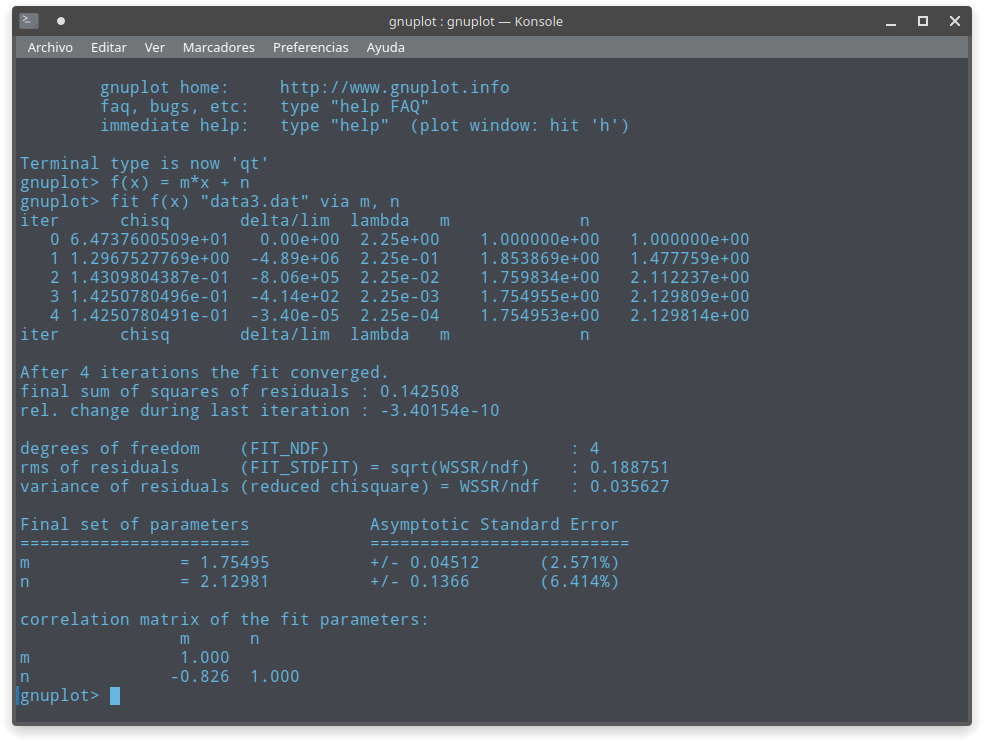
\includegraphics[scale=0.4]{Capturas/02_SalidaFit.png}
	\caption{Salida mostrada por gnuplot tras realizar un ajuste lineal.}
	\label{fig:OutputFit}
\end{figure}

Por último también nos puede interesar obtener el índice de correlación $r$ para ver la bondad del ajuste. Para ello no es necesario que usemos el comando ``fit'', simplemente tenemos que ejecutar el comando ``stats'' seguido de el nombre del fichero que estemos usando, en nuestro ejemplo es ``data3.dat''. Así pues si ejecutamos:

\begin{lstlisting}[language=Gnuplot]
stats "data3.dat"
\end{lstlisting}

Nos tendrá que mostrar una salida como la que se muestra en la figura \ref{fig:OutputStats}. Entre otra información útil que este comando nos muestra podemos observar que en la penúltima línea nos pone el índice de correlación $r$. Como ya bien sabréis un índice de correlación muy cercano a uno en valor absoluto indica que el ajuste es bueno, mientrar que si el valor no se acerca en valor absoluto a uno significa que es un mal ajuste. \textbf{Ojo:} En algunas ocasiones puede ser que gnuplot nos muestre que $r$ es igual a uno, pero no nos lo podemos tomar al pie de la letra pues una correlación perfecta es imposible. Lo más correcto sería indicar que $r \approx 1$.

\begin{figure}[h]
	\centering
	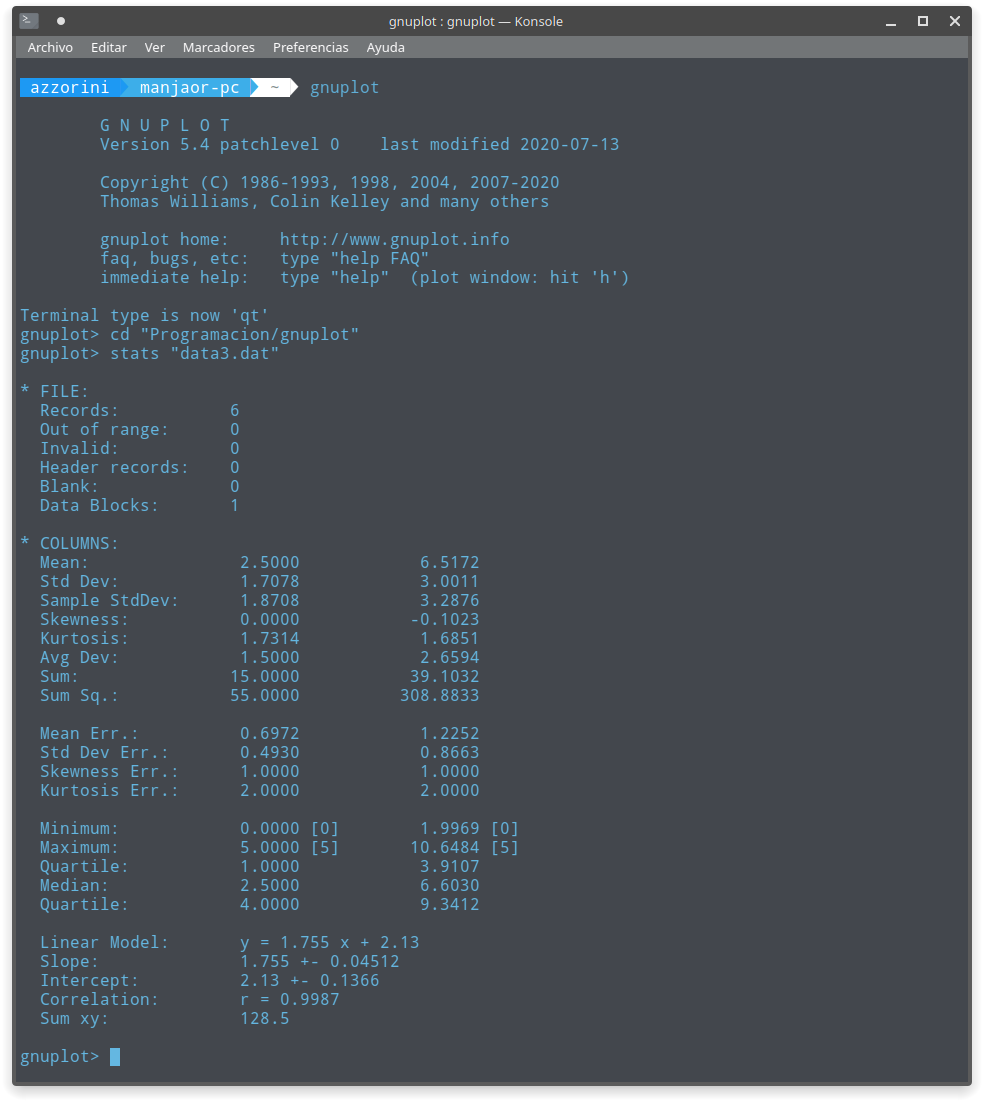
\includegraphics[scale=0.25]{Capturas/03_SalidaStats.png}
	\caption{Salida mostrada por gnuplot tras utilizar el comando ``stats''.}
	\label{fig:OutputStats}
\end{figure}

Llegado a este punto ya tenemos información suficiente para realizar cualquier tipo de ajuste lineal, obtener los valores del ajuste junto con sus errores y además poder determinar la bondad del ajuste. A continuación, explicaremos como proceder cuando queremos realizar un ajuste no lineal.

\subsubsection{Ajustes no lineales}

Gnuplot también es una potente herramienta para realizar ajustes no lineales de los datos. Al igual que para los ajustes lineales se utiliza el método ``fit''. No obstante habrá que tener otras consideraciones que pueden dificultar las operaciones y que hacen que hacer ajustes no lineales sea un arte\footnote{De hecho es aconsejable que si se pueden linealizar los datos se haga en lugar de intentar realizar un ajuste no lineal.}.\\

Imaginemos que tenemos el fichero ``data5.dat'' con el contenido que se muestra en la tabla \ref{tab:data_plot_nonlinfit}. Estos datos han sido generados usando la función $f(x) = 3e^{-2x} + 1$ a la cual se le ha introducido un cierto error para que los resultados sean más realistas. \\

\begin{table}[h]
 \centering
 \caption{Contenido fichero ``data5.dat''.}
 \vspace{10pt}
 \label{tab:data_plot_nonlinfit}
 \begin{tabular}{cccc}
  \# $x$ & $y$ & $\Delta x$ & $\Delta y$ \\
	0.00 & 4.02 & 0.08 & 0.13 \\
	1.00 & 1.34 & 0.08 & 0.07 \\
	2.00 & 1.09 & 0.08 & 0.05 \\
	3.00 & 1.04 & 0.08 & 0.05 \\
	4.00 & 0.96 & 0.08 & 0.04 \\
	5.00 & 1.01 & 0.08 & 0.03 \\
	6.00 & 0.97 & 0.08 & 0.03 \\
	7.00 & 0.95 & 0.08 & 0.05 \\
	8.00 & 0.97 & 0.08 & 0.04 \\
	9.00 & 1.02 & 0.08 & 0.03 \\
 \end{tabular}
\end{table}

En primer lugar como viendo los datos se puede observar que los datos se corresponden a una exponencial decreciente se definirá la siguiente función en gnuplot:

\begin{lstlisting}[language=Gnuplot]
f(x) = A*exp(-B*x) + C
\end{lstlisting}

Una vez definida esta función ya podremos probar a utilizar el comando ``fit'' para que ajuste las constantes que hemos definido. De esta forma y por un procedimiento completamente idéntico al empleado en el apartado \ref{subsubsec:ajusteslineales} se puede emplear el siguiente script:

\begin{lstlisting}[language=Gnuplot]
set terminal png
set output "AjusteExponencial.png"

set xrange [-0.5:10]
set yrange [0.5:4.5]

f(x) = A*exp(-B*x) + C

fit f(x) "data5.dat" via A, B, C

plot "data5.dat" w xyerr t "Datos", f(x) t "Ajuste"
\end{lstlisting}

No obstante resulta que hemos tenido bastante suerte con el ejemplo elegido porque no siempre es tan fácil. Probemos una cosa para demostrar que no es tan sencillo, en lugar de definir una exponencial negativa vamos a definirla directamente como positiva (ahora gnuplot tendría que llegar a un valor de $B$ negativo). Pero si probamos a ejecutar ese pequeño cambio veremos que el resultado que gnuplot nos devuelve es disparatado. Esto se debe a que \textbf{el resultado de los ajustes no lineales depende mucho de las condiciones iniciales que le demos.} Aunque no siempre es sencillo saber cual es el valor correcto para darle a las constantes siempre es aconsejable que sean del mismo signo al valor que creemos que va a salir y, a ser posible, del mismo orden de magnitud. Para arreglar el problema que acabamos de ocasionar al código tenemos entonces que añadir antes del fit un valor inicial de $B$ que se corresponda mejor con los valores que esperamos tener al final: 

\begin{lstlisting}[language=Gnuplot]
set terminal png
set output "AjusteExponencial.png"

set xrange [-0.5:10]
set yrange [0.5:4.5]

f(x) = A*exp(B*x) + C

B = -1
fit f(x) "data5.dat" via A, B, C

plot "data5.dat" w xyerr t "Datos", f(x) t "Ajuste"
\end{lstlisting}

Así pues hemos conseguido arreglar nuestro primer script y, de paso, hemos aprendido la importancia de las condiciones iniciales de las constantes en este tipo de ajustes.\\

Por último cabe destacar que no es tan sencillo obtener la bondad del ajuste puesto que el coeficiente de correlación solo aplica a ajustes lineales. No obstante gnuplot si nos da datos como para estimar la bondad del ajuste. En concreto nos da el valor ``reduced chisquare'' que se llama así por la distribución estadística $\chi^2$. El valor que gnuplot nos muestra nos indica un buen ajuste cuando el resultado se acerque a $1.0$ y malo cuando sea mucho menor que $1.0$ o mucho mayor\footnote{Aunque de querer obtener un mejor indicador no es tan sencillo (mejor remitirse a un libro de estadística), incluso las estimaciones de error que gnuplot muestra para ajustes no lineales son una aproximación no excesivamente buena y lo más correcto sería que los calculáramos nosotros a mano haciendo uso de estadística.}.

\subsection{Operador ternario}

Existe un operador en gnuplot que es muy importante cuando queremos definir funciones a trozos y este es llamado el operador ternario. Se llama así porque recibe tres argumentos: una condición que comprueba si es verdadera o falsa, un valor para cuando la condición es verdadera y un valor para cuando la condición es falsa. Su sintaxis es: ``(condicion ? valor\_si\_verdadero : valor\_si\_falso)''. Cabe destacar que los operadores que se pueden usar en la condición son idénticos a los que se usan en C: !, \textless , \textgreater , ==, \textless =, \textgreater =, \&\& y \textbar\textbar. Usando este operador y anidándolos se puede construir cualquier tipo de función a trozos. \\

Algunos ejemplos sencillos:

\begin{lstlisting}[language=Gnuplot]
# Funcion paso o funcion de Heaviside
H(x, a) = (x < a ? 0 : 1)

# Funcion pulso cuadrado
P(x, L) = (x > -L/2 && x < L/2 ? 1 : 0)

# Funcion a trozos cualquiera
pw(x) = (x < a ? f(x) : (x < b ? g(x) : (x < c ? h(x) : j(x))))
\end{lstlisting}

\subsection{Ajustar el sampling\label{subsec:Sampling}}

Como es evidente cuando gnuplot muestra funciones realmente no está mostrando una función continua, simplemente va tomando ciertas muestras del valor de la función y creando con esas muestras una gráfica aparentemente continua. No obstante, en algunos casos se necesitan altos niveles de detalle y nos interesa aumentar el sampling aunque eso supongo que cueste un poco más graficar la función. Para configurar el sampling haremos uso de ``set samples'' acompañado del número de valores que queremos que gnuplot tome. En el apartado \ref{subsec:Sumatorias} se muestra un ejemplo en el cual es conveniente ajustar el sampling para obtener un resultado satisfactorio.

\subsection{Sumatorias\label{subsec:Sumatorias}}

También es posible indicarle a gnuplot que se quieren realizar sumatorias lo cual puede ser útil para mostrar ciertas funciones o para procesar ciertos datos. Para indicarle a gnuplot que se quiere realizar una sumatoria se ha de usar la sentencia ``sum''. \\

La \textbf{sintaxis} de la sentencia ``sum'' es la siguiente: ``sum [variable = valor\_inicial : valor\_final] expresion''. Por ejemplo, algunas series se podrían definir de la siguiente manera:

\begin{lstlisting}[language=Gnuplot]
euler = sum [i=1:10000000] (1.0/i)**2
zenon = sum [n=1:10000] (0.5)**n
print "Serie de Euler: ", euler, " ~ ", pi**2/6
print "Serie paradoja Zenon: ", zenon, " ~ ", 1
\end{lstlisting}

Además de usarlo para obtener solo una sumatoria, que es un claro ejemplo para ver como funcionan, también se pueden usar la sumatoria para definir funciones. Un ejemplo famoso de función que se define mediante una sumatoria es la función de Weierstrass. Esta función es famosa por ser continua en todo $\mathbb{R}$ y no derivable en ningún punto. Su definición es la siguiente:
\[
	w(x) = \sum_{n=0}^{\infty} a^n \cos\left( b^n \pi x  \right) 
,\]donde $a$ y $b$ son dos constantes que se pueden elegir respetando una serie de condiciones. Una vez definida la función vamos a intentar implementarla en gnuplot, para ello definiremos una función que vamos a llamar ``weie'' y que va a recibir como parámetros la variable independiente $x$, las constantes ya antes mencionadas que vamos a llamar $wa$ y $wb$ y un entero que va a indicar hasta que término de la sumatoria contar llamado $n$, pues no podemos sumar los infinitos términos (los números se hacen tan grandes que gnuplot no puede con ellos).

\begin{lstlisting}[language=Gnuplot]
weie(x, wa, wb, n) = sum [i=0:n] wa**i*cos(wb**i*pi*x)
\end{lstlisting}

Ahora siguiendo lo que ya sabemos tendremos que definir un tipo de terminal, configurar la salida, configurar los límites, quitar la leyenda y mostrar la función. No obstante, si seguimos estos pasos y obtenemos la gráfica veremos que falta mucho detalle. Esto se debe a que se tiene que ajustar el sampling como se explicó en el apartado \ref{subsec:Sampling}. Con todo esto, el código quedaría tal que así:

\begin{lstlisting}[language=Gnuplot]
set terminal png
set output "graph_weierstrass.png"

unset key

set xrange [-2:2]
set yrange [-2:2]
set samples 1000 # Mejora los detalles de la grafica

# Parametros funcion
a = 0.5
b = 3

# Numero de sumandos a tomar
N = 500

# Funcion de weierstrass que recibe cuatro parametros:
#     x: Variable independiente
#     wa: Primer parametro
#     wb: Segundo parametro
#     n: Numero de sumandos a tomar
weie(x, wa, wb, n) = sum [i=0:n] wa**i*cos(wb**i*pi*x)

plot weie(x, a, b, N) lc "dark-red" lw 2
\end{lstlisting}

\subsection{Configurar tics\label{subsec:ConfigurarTics}}

Ya hemos visto en algunos apartados que es necesario o importante configurar los tics para ciertas cosas, como puede ser mostrar el grid. Además son útiles también en general para que la información mostrada en el gráfica sea más sencilla de leer. Primero veremos como configurar los tics mayores, algunos ajustes que se pueden hacer sobre ellos y como configurar los tics menores.\\

\textbf{Indicar los tics mayores:} Existen varias opciones para indicar los tics mayores pero todas ellas han de empezar por ``set xtics'' para configurar los tics en el eje $x$ y ``set ytics'' para configurar los tics en el eje $y$. Al igual que con el grid o con la leyenda también se pueden desactivar cambiando el ``set'' por ``unset''. Ahora bien si no indicamos nada será gnuplot quien se encargue de decidir el intervalo en el que se quiere mostrar los tics y su frecuencia. No obstante también se puede configurar esto:

\begin{enumerate}
	\item \textbf{Indicar la frecuencia:} Para indicar la frecuencia con la que se muestran los tics solo es necesario añadir un número al final que será lo que gnuplot tome por frecuencia es decir: ``set xtics 5'' mostrará un tic cada 5 unidades.
	\item \textbf{Indicar intervalo y frecuencia:} También se le puede dar a gnuplot la información sobre el intervalo en el que queremos que se muestre así como de su frecuencia. Para esto tendremos que indicar tres número separados por comas. El primero indicará el principio del intervalo, el segundo la frecuencia y el tercero el final del intervalo. Así pues si ponemos ``set ytics 0, 2, 8'' gnuplot nos mostrará tics entre $0$ y $8$ (incluidos) separados por dos unidades.
	\item \textbf{Indicar tics personalizados:} Existe también la opción de indicar los tics de una forma completamente a la carta y permitiendo el poner nombres a cada tic\footnote{No obstante, esta opción está desaconsejada puesto que si la usamos no se puede hacer uso luego de los tics menores. Existe la opción de añadir tics personalizados con ``set xtics/ytics add'' que explicaremos más adelante.}. Para indicar tics de manera personalizada tendremos que indicarlos todos metidos entre paréntesis y separados por comas. Además si queremos que un tic en concreto vaya con una etiqueta personalizada tendremos que poner una cadena de caracteres antes del número separado por un espacio en blanco. ``set xtics (1, 2, 3, 5, 6, 7, 8)'' o \textit{set ytics (``-Pi'' -pi, -2, -1, 0, 1, 2, ``Pi'' pi)} son ejemplos de esto.
\end{enumerate}

\textbf{Añadir tics personalizados:} En ocasiones además de los tics regulares que se suelen poner en cada gráfica existen valores interesantes que se quieren indicar también en los ejes. Para este objetivo en gnuplot podemos escribir ``set xtics/ytics add''. Después de esto podremos indicar los tics a añadir con el mismo formato que ya se ha explicado para los tics personalizados, es decir, se pone todo entre paréntesis y cada tic separado por comas (con la opción de añadir etiquetas para cada tic). Ejemplo: \textit{set xtics add (``-Pi'' -pi, ``Pi'' pi)}.\\

\textbf{Configurar algunas opciones:} También es posible configurar algunas opciones de los tics para mejorar su estética. Entre las distintas opciones vamos a destacar las siguientes:

\begin{enumerate}
	\item \textbf{Rotar los tics:} Existe la opción de rotar los tics añadiendo a ``set xtics/ytics/tics'' la opción ``rotate''. Esto rotará la letra de todos los tics $90^{\circ}$. En algunas terminales podremos especificar después de rotate los grados que queremos que el texto se gire.
	\item \textbf{Posición de los tics con respecto de la gráfica:} También podemos elegir si queremos que los tics se muestren dentro de la gráfica o fuera de ella. Por defecto se muestran dentro pero se puede configurar esto usando las opciones ``in'' y ``out''.
	\item \textbf{Ajustar un offset:} Existe por último otra opción a destacar sobre todo porque permite ajustar un poco los tics que se pueden descuadrar al usar la opción rotate. Por defecto indican un offset en caracteres (tanto para la x, como para la y) con respecto a la posición donde gnuplot va a mostrar los tics. Para ello solo tenemos que indicar la opción ``offset x, y''. En el ejemplo de mejorar unos tics que han sido rotados podemos imaginarnos que se han rotado los tics del eje $x$. Para hacer que las etiquetas se muestren centradas sería conveniente que se añadiera ``set xtics offset 0.5, 0''. Esto lo que hace es desplazar los tics medio caracter hacia la izquierda haciendo que se muestren centrados con respecto a las líneas\footnote{Es importante la posición en la que se ponga el offset pues si lo mezclamos con otros número como pueden ser los del intervalo a mostrar podemos tener problema, por todo ello es aconsejable poner esto siempre al final.}.
\end{enumerate}

Por último, también se pueden establecer unos tics menores. Estos se establecen con ``set mxtics/mytics'' y son unos tics de menor tamaño que aparecen sin etiqueta. Estos no permiten un alto grado de personalización, sin embargo podemos decidir cuantos intervalos (que no líneas) se van a mostrar entre cada uno de los tics mayores. Para ello simplemente hay que añadir un número al final que indicará este número de intervalos a dividir.\\

Con todo esto un buen ejemplo en el que ver muchas de las cosas que aquí se han explicado sería el de mostrar la radiación de un cuerpo negro, donde vamos a rotar los tics del eje $x$, vamos a personalizar el intervalo y la frecuencia de dichos tics y además vamos a añadir uno extra con el máximo. Por último se configurarán también los tics menores para completar lo aquí enseñado. El script es el siguiente:

\begin{lstlisting}[language=Gnuplot]
set terminal png
set output "rad_blackbody.png"

# Constantes necesarias (en el SI)
h = 6.626070150e-34
c = 299792458
k = 1.3806488e-23
b = 2.8977729e-3

# Temperatura del cuerpo negro (K)
T = 6000

# x en nm
L(x) = 2*h*c**2/(x*1e-9)**5/(exp(h*c/(x*1e-9)/k/T)-1)

unset key

set xrange [100:1300]
set xlabel "Longitud de onda (nm)"
set ylabel "Radiancia (W/sr m^3)"
set title "Radiancia de un cuerpo negro T=6000K"

set tics out # Usamos esto para aplicarlo a ambos ejes
set xtics rotate 100, 300, 1300 offset 0.5, 0

set xtics add ("Max" b/T*1e9)

set mxtics
set mytics

plot L(x) lc "dark-red" lw 2
\end{lstlisting}

\subsection{Configurar bordes}

También se puede configurar como queremos que se muestre el borde de los gráficos. Para ajustar eso utilizaremos el comando ``set border'' y para quitarlo podremos usar ``unset border''. Existen a su vez algunas opciones interesantes que se pueden configurar.

\begin{enumerate}
    \item \textbf{Posición:} La posición indica si el borde se muestra por encima o por debajo del resto de elementos de la gráfica. Por defecto es por encima que es la opción ``top'' pero también se puede cambiar para que sea por debajo usando las opciones ``back'' y ``behind''.
    \item \textbf{Estilo de líneas:} También se pueden configurar todas las opciones de estilo de líneas que ya hemos visto. Está todo explicado en el apartado \ref{subsec:EstiloLinea} así que no lo repetiremos de nuevo.
    \item \textbf{Estilo polar:} También se puede modificar el estilo del borde para cuando se quiera mostrar una gráfica en formato polar. Para ello se tiene que añadir la opción ``polar''.
\end{enumerate}

\subsection{Estilos de puntos\label{subsec:EstiloPuntos}}

Al igual que con las líneas cuando se muestra una gráfica con puntos también se puede personalizar los puntos a nuestro gusto. En este apartado vamos a ver los diferentes opciones que tenemos para personalizar nuestras gráficas, en concreto: tamaño de puntos, colores de puntos y tipos de puntos.\\

Primero de todo ya hemos visto que los datos se muestran por defecto con puntos cuando estos son introducidos de un fichero, no obstante, también podemos forzar a que una función cualquiera se muestre con puntos usando la opción ``with points'' (que podemos abreviar por ``w p''). Dicho esto veamos qué se puede personalizar en las gráficas que se muestran con puntos:

\begin{enumerate}
	\item \textbf{Tamaño de puntos:} Se puede personalizar el tamaño de los puntos usando la opción ``pointsize'' (o su forma corta ``ps'') seguido de un número real que indicará el tamaño del punto en  cuestión: ``plot x w p ps 2''.
	\item \textbf{Color de los puntos:} También se puede configurar el color con el que se muestran los puntos y, aunque esto resulte un poco irónico, el color de los puntos se especifica con la opción ``linecolor'' (o más conciso ``lc'') que es lo mismo que se usa para cambiar el color a las líneas. Esta opción se puede manejar de la misma forma que se manejan los colores para las líneas (ver apartado \ref{subsec:EstiloLinea}).
	\item \textbf{Tipo de puntos}: También se puede configurar el tipo de dibujo que se quiere que aparezca sobre cada punto: cruces, triángulos, círculos, cuadrados\ldots Para ello se utilizará la opción ``pointtype'' (o ``pt'') seguida de un número entero que indicará el tipo de punto a poner. Los tipos de puntos que se tienen cambian de una terminal a otra pero se pueden consultar viendo la salida del comando ``test''. Por ejemplo: ``plot x w p pt 5''.
\end{enumerate}

Un ejemplo que puede mostrar todo esto en acción a la vez sería el siguiente para mostrar una gaussiana:

\begin{lstlisting}[language=Gnuplot]
set terminal png
set output "gaussiana.png"

set xrange [-10:10]
set yrange [0:1.2]

set samples 30

plot exp(-x**2/10) w p ps 2 pt 7 lc "dark-red"
\end{lstlisting}

Al igual que las líneas también se pueden definir estilos propios de líneas usando ``set linestyle'' junto con las propiedades del punto que queramos. Si además se quiere definir estilo de línea y de punto se pueden simplemente configurar ambas en el mismo estilo de línea y gnuplot se encargará de usar la información pertinente. Al igual que con las líneas para usar el estilo que se haya configurado se añadirá ``ls [numero\_de\_estilo]''. Para refrescar los estilos de línea ver el apartado \ref{subsec:EstiloLinea}.

\subsection{Flechas y segmentos}

También existe la opción de ajustar flechas y líneas que vayan de dos puntos completamente a nuestra decisión. Esto puede ser de gran interés pues puede ayudar a que nuestras gráficas sean más sencillas de entender. Para ello usaremos la siguiente sintaxis: ``set arrow [index] from x1,y1 to x2,y2 [options]''. Donde [index] es un número arbitrario que nos sirve para identificar la flechas y poder modificarlas en un futuro o incluso borrarlas usando ``unset arrow [index]'', los valores x1, y1, x2 e y2 indican las coordenadas del punto inicial y final de la flecha y finalmente en [options] se pueden indicar una serie de propiedades de la flecha:

\begin{enumerate}
	\item \textbf{Cambiar la flecha por un segmento:} Por defecto lo que se muestra es una flecha, sin embargo, si especificamos la opción ``nohead'' no se nos mostrará la flechita final quedando un segmento solamente.
	\item \textbf{Cambiar la posición o el número de flechas:} También en lugar de quitar directamente las flechas se puede cambiar su posición. La posición por defecto se corresponde con la opción ``head''. Si queremos que se muestre al revés se puede utilizar la opción ``backhead''. Finalmente, si queremos que se muestren flechas en ambos lados se puede utilizar la opción ``heads''.
	\item \textbf{Cambiar el estilo de las flechas:} También es posible cambiar los estilos de las flechas indicando una opción de entre las siguientes: ``filled'', ``nofilled'', ``noborder'', ``empty''. Las opciones no tienen mucho que explicar pero es aconsejable que las probéis para ver como funcionan.
	\item \textbf{Cambiar el tamaño de las flechas:} También es posible cambiar el tamaño de las flechas mediante la opción ``size (tamaño\_flecha), (ángulo\_flecha) [, (ángulo\_trasero)]. Donde solo es obligatorio especificar los dos primeros números que son el tamaño de la flecha y el ángulo que forma en su punta en grados. Si se añade una coma y se indica otro ángulo en grados se puede configurar el ángulo que se muestra por el lado de la flecha que corta con el segmento. Es necesario darle un valor a este ángulo suficiente para que no corte con la punta de la flecha, un valor de entorno a $60^{\circ}$ puede estar bien.
	\item \textbf{Ajustar la posición de la flecha:} Podemos elegir si queremos que la flecha se muestre encima de las cosas que queremos mostrar usando la opción ``front'' o debajo de todo usando la opción ``back''.
	\item \textbf{Ajustar el estilo de la flecha:} También se puede configurar en la flecha todo lo que tiene que ver con estilos de línea: ``lw'', ``lc'', ``dt''\ldots Todo esto se hace añadiendo las opciones igual que se hace con las líneas (ver apartado \ref{subsec:EstiloLinea}).
\end{enumerate}

\subsection{Objetos\label{subsec:Objetos}}

Al igual que las flechas también es posible mostrar algunos tipos de objetos que pueden ser de utilidad en ciertas ocasiones, en concreto se pueden mostrar: rectángulos, círculos, elipses y polígonos. Todos ellos se han de mostrar usando el comando ``set object'', tras este comando podremos poner un número que nos sirva para identificar el objeto, después pondremos el tipo de objeto que se quiere poner y por último las opciones de este objeto. Ahora procederemos a explicar las características básicas de cada tipo de objeto:

\begin{enumerate}
	\item \textbf{Rectángulos:} Su tipo de objeto es ``rectangle'' (que se puede abreviar por ``rect''). Existen dos formas de declararlos. La primera es dando dos puntos, primero el de la izquierda del rectángulo y después uno de la derecha\footnote{Esto se puede invertir usando ``rto'' en lugar de ``to''.}. Para ello se escribirá ``set object 1 rect from x1,y1 to x2,y2''. También existe la forma de indicar el centro del rectángulo y después su anchura y su altura. Para esto se usará: ``set object 2 rect at x,y size ancho,alto''.
	\item \textbf{Círculos:} Su tipo es ``circle''. Existe una única forma de declararlo que es indicando su centro y después su radio: ``set object 1 circle at x,y size radio''. También se puede dibujar solamente una sección angular del círculo para ello se indicará la opción ``arc [inicio:fin]'' donde inicio y fin son dos ángulos en grados que se tomarán siempre en el sentido contrario de las agujas del reloj. Si los ejes no están en la misma escala el círculo en realidad se tendría que mostrar como una elipse pero el radio se toma siempre en las coordenadas horizontales por lo que esto no pasará, para ello se tiene el tipo elipse.
	\item \textbf{Elipse:} Su tipo es ``ellipse''. La única forma de declararlo es indicando su centro, su anchura y su altura. Para ello se usará la siguiente sintaxis: ``set object 1 ellipse at x,y size ancho,alto''. También se puede indicar la orientación de la elipse mediante la opción ``angle orientación'' donde orientación es un ángulo en grados. Por último una opción también bastante interesante es la de ajustar las unidades. Por defecto se usarán las unidades del eje $x$ para el ancho y las del eje $y$ para el alto pero esto se puede cambiar usando la opción: ``units xx/xy/yy''. De hecho si se va a rotar la elipse y la escala de los ejes es distinta se perderá la proporción entre el eje menor y el eje mayor al rotarla de usar la opción ``units xy''.
	\item \textbf{Polígonos:} Por último también se pueden hacer polígonos a nuestra voluntad usando el tipo ``polygon''. Para indicar el polígono simplemente indicaremos sus vértices escribiendo: ``set object 1 polygon from x1,y1 to x2,y2 to x3,y3 \ldots to xn,yn'', para cerrar el polígono es importante que el último vértice que se indique coincida con el primero. Por ejemplo podríamos pintar un triángulo de la forma: ``set object 2 polygon from 0,3 to 1.5, 0 to -1.5,0 to 0,3''.
\end{enumerate}

También existen un par de opciones para ajustar la apariencia de los objetos que son de interés:

\begin{enumerate}
	\item \textbf{Estilo de relleno:} Se puede indicar el estilo de relleno mediante la opción ``fillstyle'' (o simplemente ``fs''). Si queremos que no se muestre ningún relleno se puede usar la opción ``empty'' si queremos que se rellene con un color sólido podemos usar la opción ``solid'' seguida de un número que indica la densidad del color donde $1.0$ indica todo el color y $0.0$ indica el mismo color que el fondo de la gráfica. Además si se indica la opción ``transparent solid'' esta densidad se interpretará como la opacidad del relleno. Por último también se puede indicar la opción ``pattern'' seguido de el número del patrón que queremos que se muestre. Podemos ver los patrones disponibles en la terminal que usemos viendo la salida de ``test''. También se pueden configurar los bordes usando la opción ``border'' seguido de un tipo de línea indicado por ``lt'' o de un color indicado por ``lc''. En caso de no querer bordes se puede usar la opción ``noborder''.
	\item \textbf{Color de relleno:} También se puede indicar el color de relleno usando la opción ``fillcolor'' (o ``fc'') seguido de un indicador de color válido (ver apartado \ref{subsec:EstiloLinea}).
	\item \textbf{Ancho y patrón de las líneas:} También se puede indicar el ancho y el patrón de las líneas mediante las opciones ``lw'' y ``dt'' tal y como se indicó en el apartado \ref{subsec:EstiloLinea}.
	\item \textbf{Posición del objeto:} También se puede indicar la posición del objeto usando las opciones ``front'', ``back'' y ``behind''. La opción ``front'' sitúa el objeto delante de todas las cosas que se vayan a graficar. La opción ``back'' sitúa el objeto detrás de todo lo que se vaya a graficar. Por último la opción ``behind'' sitúa el objeto en el fondo de todo (incluyendo ejes, tics, títulos\ldots). Esta opción tiene una utilidad muy interesante y es el de cambiar el color del fondo. Para ello lo que se tiene que hacer es especificar un rectángulo que vaya de una esquina a otra de la pantalla: ``set object 1 rect from screen 0,0 to screen 1,1 behind''\footnote{La palabra ``screen'' antes de que se indiquen las coordenadas nos indica que queremos que se tomen las coordenadas con respecto a la pantalla donde 0,0 es la esquina inferior izquierda y 1,1 es la esquina superior derecha. Existen también otras coordenadas de interés como ``graph'' que funciona igual que esta pero solo en el recinto de graficado.}.
\end{enumerate}

Con esto último que se ha comentado se puede hacer un pequeño script para graficar algo en \textit{modo oscuro}:

\begin{lstlisting}[language=Gnuplot]
set terminal png
set output "oscuro.png"

set object 1 rectangle from screen 0,0 to screen 1,1\
	behind fc "black"
set border lc "white" # Pone los bordes blancos
unset key

plot x lw 2 lc "red"
\end{lstlisting}

\subsection{Etiquetas}

Otra de las cosas que gnuplot nos permite es la colocación de etiquetas que permitan añadir una pequeña explicación adicional sobre lo que queremos mostrar en nuestra gráfica. Esto se hace mediante el comando ``set label''. La sintaxis es básicamente: ``set label [etiqueta] [texto] at [posicion] [opciones]'', donde la etiqueta es opcional y es un número que sirve para editar el label en otros comandos (o borrarlo usando ``unset label [etiqueta]''), el texto es el contenido que queremos que muestre la etiqueta, posición es el punto donde queremos que se empiece a escribir el texto en el formato x,y y finalmente podemos añadir una serie de opciones que permiten modificar un poco la etiqueta. \textbf{Ejemplo:} \textit{set label 1 ``Prueba'' at 2,3}. \\

Ahora que ya conocemos la sintaxis básica de como colocar una etiqueta podemos aprender algunas opciones interesantes que nos pueden servir para personalizar un poco nuestras etiquetas:

\begin{enumerate}
    \item \textbf{Posición del texto con respecto al punto:} Una de las cosas que se pueden elegir es donde queremos que se escriba el texto con respecto al punto que hemos indicado. Por defecto el texto dejará al punto dado a la izquierda pero esto se puede cambiar con las opciones ``right'', ``center'' o ``left''.
    \item \textbf{Posición de la etiqueta:} Otra de las cosas que hay que decidir es donde colocar la etiqueta con respecto al resto de los elementos de la gráfica. Por defecto las etiquetas se sitúan al fondo de todo (opción ``back''). Pero en algunas ocasiones, en especial cuando se tiene una densidad de datos alta, es normal que se quiera llevar la etiqueta al frente para que así los datos no la oculten. Para ello usaremos la opción ``front''.
    \item \textbf{Rotar:} En algunas terminales también podemos elegir la opción de rotar las etiquetas. Por defecto se marca la opción ``norotate'' que hace que el texto se escriba en horizontal. Si se especifica la opción ``rotate'' el texto se escribirá en vertical. Finalmente, si se escribe ``rotate by [angulo]'' se rotará el texto según el valor indicado en angulo teniendo en cuenta que es un valor en grados.
    \item \textbf{Cambiar la fuente:} También existe la opción de cambiar la tipografía y su tamaño mediante la opción ``font''. Si no se indica lo contrario su valor es ``default'' que significa que es el mismo que en el resto de la gráfica. No obstante se puede indicar un string con el nombre de la fuente que se quiere usar, por ejemplo: \textit{font ``Roman''}. También se puede indicar el tamaño de la fuente añadiendo después del nombre de la fuente una coma junto con el valor deseado: \textit{font ``Roman, 14''}.
    \item \textbf{Color del texto:} Esto es algo que realmente se puede aplicar a todo lo que tenga un cierto texto. La opción a indicar es ``textcolor'' (o abreviado ``tc'') seguido de un color en el formato que ya hemos visto en el apartado \ref{subsec:EstiloLinea}.
    \item \textbf{Offset:} También se puede indicar un offset antes de mostrar el texto que puede ser útil en algunos casos. Para ello se escribirá ``offset x,y'' donde los valores de $x$ e $y$ indican el número de caracteres a moverse antes de empezar a escribir texto.
\end{enumerate}

\subsection{Texto con formato\label{subsec:TextoFormateado}}

En algunas ocasiones queremos que las gráficas muestren cierta información relacionada con algunas variables que use nuestro script de gnuplot. Esto es posible gracias a la opción ``sprintf''. Esta función recibe una cadena de caracteres que indica el formato que se desea, en este formato se puede indicar que aparezcan unas ciertas variables. Después se le pasarán a la función ordenadamente todas las variables que se quieran utilizar.\\

El formato para especificar las variables coincide con el del lenguaje de programación C. Pero básicamente todos empiezan por el caracter ``\%'' seguido de una letra que indica el tipo de variable. Las letras que más vamos a usar en el día a día son:

\begin{enumerate}
	\item \textbf{\%d}: Entero.
	\item \textbf{\%u}: Entero sin signo.
	\item \textbf{\%f}: Número decimal.
	\item \textbf{\%e}: Número decimal en notación científica.
	\item \textbf{\%g}: Número decimal en la representación más corta entre \%f y \%e.
	\item \textbf{\%c}: Caracter.
	\item \textbf{\%s}: Cadena de caracteres.
\end{enumerate}

Además en el caso se los números se puede especificar una ``h'' delante para indicar que son números cortos y una ``l'' delante para indicar que son números largos. Esto se refiere a la cantidad de memoria que se reserva para las variables y repercute en el tamaño máximo y la precisión que estos números pueden llegar a tener. Por último, en los números también se puede indicar al principio de todo la precisión que se quiere tener poniendo un punto seguido del número de decimales que se quieren tomar. Un ejemplo sería por ejemplo mostrar un número real con tres decimales: ``\%.3f''. \\

Un ejemplo claro de todo esto sería el modificar el script del apartado \ref{subsec:ConfigurarTics} para que muestre la temperatura del cuerpo negro y su máximo de forma automática:

\begin{lstlisting}[language=Gnuplot]
set terminal png
set output "rad_blackbody.png"

# Constantes necesarias (en el SI)
h = 6.626070150e-34
c = 299792458
k = 1.3806488e-23
b = 2.8977729e-3

# Temperatura del cuerpo negro (K)
T = 6000

# x en nm  
L(x) = 2*h*c**2/(x*1e-9)**5/(exp(h*c/(x*1e-9)/k/T)-1)

unset key

set xrange [100:1300]
set xlabel "Longitud de onda (nm)"
set ylabel "Radiancia (W/sr m^3)"
set title sprintf("Radiacion de un cuerpo negro T=%.0fK", T)

set tics out # Usamos esto para aplicar cosas a ambos ejes
set xtics rotate 100, 300, 1300 offset 0.5, 0

maximo = b/T*1e9
set xtics add (sprintf("%.0f", maximo) maximo)

set mxtics
set mytics

plot L(x) lc "dark-red" lw 2
\end{lstlisting}

\subsection{Cambiar el formato de los tics}

También existe la opción de cambiar el formato que gnuplot nos muestra para los tics de los ejes $x$ e $y$. Esto se realiza mediante la instrucción ``set format x/y'' seguido del formato en el que queremos que se muestren. Para indicar el formato se va a utilizar una notación muy parecida a la del apartado \ref{subsec:TextoFormateado}, usando los símbolos \% junto con el número de decimales a tomar de forma opcional y el tipo de valor que se quiere mostrar. De hecho, nos sirven los formatos ``\%f'' para números decimales, ``\%e'' para notación científica y ``\%g'' para lo más corto de ambos. Todo esto ya ha sido explicado en el apartado \ref{subsec:TextoFormateado}. Sin embargo, se pueden usar también otras opciones que nos permiten construir un formato más personalizado. Las opciones a destacar son:

\begin{enumerate}
	\item \textbf{\%t:} Devuelve la mantisa del valor en base 10.
	\item \textbf{\%T:} Devuelve la potencia en base 10.
	\item \textbf{\%l:} Devuelve la mantisa del valor en la base logarítmica actual.
	\item \textbf{\%L:} Devuelve la potencia en la base logarítmica actual.
	\item \textbf{\%s:} Devuelve la mantisa en la base logarítmica actual en \textit{potencias científicas}\footnote{Para gnuplot lo que significan las potencias científicas es que la potencia es siempre múltiplo de 3, se considera así por la comodidad para el tema de las unidades.}.
	\item \textbf{\%S:} Devuelve la potencia en la base logarítmica actual usando potencias científicas.
	\item \textbf{\%c:} Devuelve un caracter que sirve para remplazar la potencia científica por un caracter que indica el múltiplo correspondiente.
	\item \textbf{\%P:} Devuelve el valor como múltiplo de $\pi$.
\end{enumerate}

Así pues, algunos ejemplos de formatos podrían ser:

\begin{lstlisting}[language=Gnuplot]
set format x "%.2g"
set format y "%.2t 10^{%T}"
set format x "%.3s*10^{%S}"
set format y "%.4s % cm"
\end{lstlisting}

\subsection{Ajustar escala logarítmica}

En algunas ocasiones es de gran utilidad establecer una escala logarítmica en alguno de los ejes para establecer de forma más clara la información que se muestra. La sintaxis es muy sencilla lo único que hay que hacer es poner ``set logscale [ejes] [base]'' donde en los ejes podemos poner $x$, $y$ o $xy$; según a los ejes a los que se lo queramos aplicar. Finalmente se podrá añadir de forma opcional la base en la que se quiere tomar la escala logarítmica, si no se indica nada gnuplot entenderá que por defecto la base es diez. De querer quitar la escala logarítmica se puede hacer con ``unset logscale [ejes]''. Si no se indica nada sobre los ejes se quitarán las de todos los ejes.\\

Uno de los principales usos de las escalas logarítmicas además de ver cierta información con más detalle es el hecho de que las funciones exponenciales en escala logarítmica se ven como líneas rectas lo cual se puede observar en el siguiente ejemplo:

\begin{lstlisting}[language=Gnuplot]
set terminal png
set output "LogEsc.png"

set logscale y
set yr [1:1e5]

plot exp(x)
\end{lstlisting}

\subsection{Estilos de graficado útiles}

Hasta ahora hemos visto fundamentalmente tres estilos de graficado: con líneas, con puntos y con errores. No obstante existen una gran cantidad de estilos con los que podemos mostrar la información. En el manual de gnuplot que se adjunta en la documentación \cite{gnuplot-5.4-doc} encontramos una sección de 25 páginas dedicada exclusivamente a estos estilos en los que podemos observar una gran variedad. Sin embargo, en este apartado nos centraremos en aquellos que se ven más prácticos en nuestro día a día dejando de lado una gran cantidad de ellos.

\subsubsection{Mostrar con cajas}

Esta opción lo que nos permite es mostrar los datos como si se tratara de un histograma y se trata de la opción ``with boxes'' que podemos añadir al comando plot. Solo son necesarias dos columnas, una para la $x$ y otra para la $y$. Después del plot también podemos especificar el estilo de relleno usando ``fs'' y ``fc'' al igual que vimos en el apartado \ref{subsec:Objetos}. Imaginemos ahora que tenemos los datos mostrados en la tabla \ref{tab:FicheroGauss}. \\

\begin{table}[h]
	\centering
	\caption{Contenido del fichero ``gauss.dat''.}
	\label{tab:FicheroGauss}
	\begin{tabular}{cc}
	\# $x$ & $y$ \\
	-1.0 & 0.00193045413622771 \\
	0.0 & 0.0183156388887342 \\
	1.0 & 0.105399224561864 \\
	2.0 & 0.367879441171442 \\
	3.0 & 0.778800783071405 \\
	4.0 & 1.0 \\
	5.0 & 0.778800783071405 \\
	6.0 & 0.367879441171442 \\
	7.0 & 0.105399224561864 \\
	8.0 & 0.0183156388887342 \\
	9.0 & 0.00193045413622771 \\
	10.0 & 0.00012340980408668
	\end{tabular}
\end{table}

Si se quieren mostrar estos datos usando el estilo indicado podríamos hacer uso del siguiente script:

\begin{lstlisting}[language=Gnuplot]
set terminal png
set output "gausiana.png"

unset key

plot "gauss.dat" w boxes fs solid 1.0\
	border lc "black" lw 1.5 fc "dark-red"
\end{lstlisting}

\newpage

\subsubsection{Mostrar con cajas y errores}

Como ya se ha comentado anteriormente en muchas ocasiones el uso de errores es muy importante y esto no es una excepción cuando se trata de los histogramas. Para ello utilizaremos la opción ``with boxerr'' que necesita que le pasemos datos de tres columnas en el siguiente orden: valor de $x$, valor de $y$, error de $y$. No es necesario el error en el eje $x$ pues es algo que ya se indica por la separación entre los valores de $x$ que se dan.\\

Imaginemos que se quiere mostrar con este estilo el contenido del fichero ``gauss1.dat'' que se muestra en la tabla \ref{tab:FicheroGaussErrores}.

\begin{table}[h]
	\centering
	\caption{Contenido del fichero ``gauss1.dat''.}
	\label{tab:FicheroGaussErrores}
	\begin{tabular}{ccc}
	\# $x$ & $y$ & $\Delta y$ \\
	-1.0 & 0.0019 & 0.0009 \\
	0.0 & 0.018 & 0.008 \\
	1.0 & 0.11 & 0.03 \\
	2.0 & 0.37 & 0.05 \\
	3.0 & 0.78 & 0.07 \\
	4.0 & 1.00 & 0.09 \\
	5.0 & 0.78 & 0.07 \\
	6.0 & 0.37 & 0.05 \\
	7.0 & 0.11 & 0.03 \\ 
	8.0 & 0.018 & 0.008 \\
	9.0 & 0.0019 & 0.0009
	\end{tabular}
\end{table}

Para mostrar el contenido de este archivo en el estilo deseado podemos utilizar un script parecido al siguiente:

\begin{lstlisting}[language=Gnuplot]
set terminal png
set output "gausiana_error.png"

unset key

plot "gauss1.dat" w boxerr fs solid 1.0\
	border lc "black" lw 1.5 fc "dark-green"
\end{lstlisting}

\subsubsection{Curvas llenas}

En algunas ocasiones aunque sea por mera estética puede ser interesante usar un estilo que llena con un cierto estilo de relleno una cierta parte de la gráfica. Esto queda especialmente bien cuando se muestran ciertas funciones como puede ser una gaussiana y puede servir también para indicar el error de una gráfica que se quiera mostrar con líneas. La opción que tenemos que usar es ``with filledcurves'' y también podemos especificar varios tipos de opciones de interés:

\begin{enumerate}
	\item \textbf{closed:} Esta opción sirve para tratar los datos que se introduzcan (ya sean dos columnas o una función) como un polígono (que tratará gnuplot de cerrar si no se cierra él mismo).
	\item \textbf{y=[valor]:} Le indica a gnuplot que rellene el espacio entre los datos o la función introducida y la recta horizontal indicada por el valor numérico que se dé.
	\item \textbf{above:} Usado en combinación con ``y=[valor]'' solo rellena la sección por encima de la recta indicada.
	\item \textbf{below:} Lo mismo que ``above'' pero con la sección por debajo de la recta indicada.
\end{enumerate}

Así pues un ejemplo para mostrar algunas de las cosas aquí aprendidas podría ser el siguiente script:

\begin{lstlisting}[language=Gnuplot]
set terminal png
set output "llenando_curvas.png"

gauss(x,m,s) = exp(-(x-m)**2/2/s)

unset key

plot gauss(x,0,4) w filledcurves below y=1 fc "orange",\
	0.5*gauss(x,0,1) w filledcurves fc "dark-green"
\end{lstlisting}

Si se le pasan tres columnas a este estilo gnuplot tomará las dos últimas columnas como dos funciones que depende de la primera de ellas y mostrará la región que hay entre ambas.Como ya se ha dicho antes esto también sirve para mostrar el error en un gráfico que se quiere mostrar con una línea. Para ello se ploteará por un lado la gráfica con líneas y por otro la región con el error\footnote{Este truco también se puede usar para otras cosas, por ejemplo si quisiéramos mostrar una línea pero mostrar también barras de errores solo tendríamos que mostar por un lado la gráfica con líneas y por otro la gráfica con errores en el eje $y$ usando un tamaño de punto nulo.}. Supongamos que se tiene un archivo con tres columnas que son el valor de $x$, el valor de $y$ y el error de $y$. En este caso se usará el archivo ``gauss1.dat'' que puedes ver en la tabla \ref{tab:FicheroGaussErrores}. El script para mostrarlo con líneas y una zona sombreada para el error sería:

\begin{lstlisting}[language=Gnuplot]
set terminal png
set output "ErrorSombreado.png"

plot "gauss1.dat" u 1:($2-$3):($2+$3) w filledcurves\
	fs solid 0.25 fc "dark-red" t "Zona error",\
	"" w l lw 2 lc "dark-green" t "Datos"
\end{lstlisting}

\subsubsection{Líneas con errores}

Aunque ya se ha comentado que esta opción realmente se podría construir usando dos opciones que ya conocemos es mucho más cómodo tenerlo todo agrupado en una única opción. Existen tres tipos de estilos: ``yerrorlines'', ``xerrorlines'' y ``xyerrorlines''. Lo que suele ser más normal es el uso de ``yerrorlines'' pero las tres funcionan de una manera muy parecida. Para las dos primeras solo es necesario pasar tres columnas: el valor de $x$, el valor de $y$ y el error de $x$ o de $y$ según hayamos elegido un estilo u otro. Para la última opción es necesario indicar cuatro columnas pues tenemos que pasarle los dos errores. Con respecto al estilo y las opciones no hay nada nuevo ya que no hayamos visto en las secciones sobre estilos de líneas y estilos de puntos (ver \ref{subsec:EstiloLinea} y \ref{subsec:EstiloPuntos}).

\subsection{Cambiar fuente}

Otra de las opciones interesantes que gnuplot nos ofrece es la de cambiar la fuente con la que gnuplot muestra todos los textos de nuestras gráficas. Existen dos maneras de realizar esto, lo que sí es siempre igual es el formato en el que se tiene que indicar la fuente que es un string donde venga en primer lugar el nombre de la fuente y, opcionalmente, una coma y el tamaño de dicha fuente: ``Roman'' o ``Roman, 14'' son buenos ejemplos de ello. Ahora bien las opciones para cambiarla son:

\begin{enumerate}
	\item \textbf{Sin modificar el tipo de terminal:} Esta opción se puede hacer en cualquier momento sin modificar el tipo de terminal que estamos usando. La sintaxis es: ``set termoption font [fuente]'' donde la fuente viene dada en el formato ya indicado.
	\item \textbf{Al modificar el tipo de terminal:} También existe la opción de cambiarlo directamente al fijar el tipo de terminal simplemente añadiendo al final la opción ``font [fuente]''. La sintaxis final sería: ``set terminal [tipo\_de\_terminal] font [fuente]''.
\end{enumerate}

\subsection{Tipos de terminales\label{subsec:TiposTerminales}}

Existen muchos tipos distintos de terminales. Cada tipo está destinado a producir un tipo de salida distinto, de momento los tipos de terminales que hemos visto son el que nos marca gnuplot por defecto al abrirlo (que puede variar en función de la versión de gnuplot que usemos pero puede ser ``qt'', ``wxt'' o similares). Este tipo de terminal está pensado para usarla directamente en gnuplot pues produce una salida a una ventana nueva que nos muestra la gráfica y nos permite hacer una pequeña serie de cosas con ella. También hemos estado usando la terminal ``png'' para producir una salida a imágenes png. En este apartado veremos otras terminales que también pueden ser de gran interés.

\subsubsection{Mejor terminal para \LaTeX}

Una de las mejores terminales para cuando vayamos a incluir las gráficas en un documento en el que usamos \LaTeX\ es ``epslatex''. La salida de este documento se ha de configurar como un fichero de \LaTeX\ con la extensión ``.tex''. La potencia que tiene este tipo de terminal es que produce dos ficheros de salida. El primer fichero es el que hemos indicado que es un fichero de \LaTeX\ que guarda toda la información sobre el texto que se quiere mostrar y el segundo es una imagen en formato EPS que guarda la gráfica en sí. Esto significa que \textbf{se pueden usar todas las funciones de \LaTeX\ en el texto a mostrar.} \\

El único detalle es que para incluir este tipo de gráfica en nuestros documentos no se puede usar ``\textbackslash includegraphics'' como estamos acostumbrados con las gráficas normales. En su lugar tendremos que usar el comando ``\textbackslash input'', que se usa en la forma ``\textbackslash input\{fichero.tex\}'' donde fichero es el nombre del archivo que hayamos puesto en gnuplot. Usar ``input'' en lugar de ``includegraphics'' tiene también la desventaja de que no se puede cambiar el tamaño de la gráfica tan fácilmente. Para poder modificar dicho tamaño podemos usar: ``\textbackslash resizebox\{.95\textbackslash linewidth\}\{!\}\{\textbackslash input\{fichero.tex\}\}''\footnote{Aunque la solución es relativamente sencilla en el caso de \LaTeX\ no se puede decir lo mismo de LyX. El consejo sencillo sería usar directamente \LaTeX , no obstante, en teoría es posible llegar a configurar LyX para que muestre estos tipos de archivo pero esta explicación excede los límites de este texto.}, donde además el .95 que acompaña a \textbackslash linewidth se puede cambiar por cualquier otro valor que se quiera. \\

Un ejemplo sencillo que podemos ver para apreciar la potencia de esta terminal es el siguiente script\footnote{Se tienen que poner dos ``\textbackslash'' en los strings porque si fuera solo uno gnuplot se pensaría que queremos introducir algún caracter especial.}:

\begin{lstlisting}[language=Gnuplot]
set terminal epslatex
set output "latex.tex"

set xr [-6:6]
set yr [0:1.4]

gauss(x,m,sg) = exp(-(x-m)**2/2/sg)

H(x, a) = (x < a ? 0 : 1)

plot (1-H(x,1))*gauss(x,0,2) w filledcurves\
    fc "dark-green" t "$\\int_{-\\infty}^xf(y)dy$",\
    gauss(x,0,2) lw 4 lc "black" t "$f(y)$"
\end{lstlisting}

En algunas ocasiones nos puede ser interesante meter un pequeño preámbulo a nuestra gráfica en la que poder incluir algún paquete (aunque la gráfica tomará los paquetes también de nuestro documento) y en el que poder definir algunos comandos de \LaTeX . Para indicar este pequeño preámbulo al fijar el tipo de terminal deberemos añadir la opción ``header'' seguido de un string con todo lo que queramos incluir: \textit{set terminal epslatex header ``preambulo''}.

\subsubsection{Terminal para gráficos vectoriales}

Otra buena opción para nuestra terminal es una que nos devuelva una gráfica en formato vectorial. La ventaja de este formato es que se pueden cambiar sus dimensiones sin que eso afecte a la calidad de la imagen. Este tipo de terminal se conoce como ``svg'' y produce archivos de salida con la extensión ``.svg''. Para incluir este tipo de archivos en \LaTeX\ se tiene que usar el paquete ``svg'' (meter ``\textbackslash usepackage\{svg\}'' en el preámbulo) y en concreto la función ``\textbackslash includesvg''.

\subsubsection{Terminales cairo}

Existen también un tipo de terminales terminadas en cairo, en concreto algunas que pueden aportar algo nuevo a esta lista son ``pdfcairo'' y ``pngcairo''. La salida que producen estas terminales son archivos de imagen normales pero cuentan con la ventaja de que utilizan una mejor gestión de las fuentes que nos facilita mucho más su personalización y su adaptación al estilo que les deseamos dar.

\subsection{Cambiar tamaño de la terminal}

La mayoría de las terminales en las versiones modernas de gnuplot tienen una opción muy últil conocida como ``size''. Esta opción indica el tamaño del canvas sobre el que se van a mostrar nuestras gráficas. Simplemente después de indicar el tipo de terminal con ``set terminal [TerminalType]'' se le añade la opción ``size x,y'' donde $x$ e $y$ indican el tamaño en píxeles de la salida a producir. ``set term [TerminalType] size x,y''.

\subsection{Estadísticas de fichero}

En alguna ocasión ya hemos hecho uso del comando ``stats'' pero en este apartado vamos a aprender a sacarle un mayor partido. Además de mostrar una gran cantidad de información por pantalla el comando ``stats'' también guarda una gran cantidad de variables relacionadas con la(s) columna(s) que le hayamos pasado. Estas variables se pueden usar luego en nuestro script. La sintaxis básica es: \textit{stats ``datafile.dat''}. Aunque sobre esto se puede añadir una serie de cosas de interés.  \\

Existen tres formas de indicarle a ``stats'' los datos que queremos procesar. La primera es poner ``u'' seguido del número de columna a procesar. La segunda opción es también indicando la opción ``u'' pero añadiendo dos números de columna separados por ``:'', en este caso interpretará que la primera columna es la $x$ y la segunda la $y$. La tercera es usar la opción ``matrix'' que tratará todo nuestro fichero como una gran matriz.

Como ya se ha mencionado antes existen un sinfín de variables que el comando ``stats'' crea al ser llamado. Cabe destacar que en caso de que se le llame pasándole dos columnas la información relativa a la primera se obtendrá añadiendo ``\_x'' al final y la relativa a la segunda se obtendrá usando ``\_y''. En la tabla \ref{tab:VariablesStats} se pueden ver algunas de las variables más destacables. \\

\begin{table}[h]
	\centering
	\caption{Variables a destacar creadas por el comando ``stats''.}
	\label{tab:VariablesStats} 
	\vspace{10pt}
	\begin{tabular}{l|l}
		\ \ \ \ \ \ \ \textbf{Variable} & \ \ \ \ \ \ \ \ \ \ \ \ \ \ \  \ \ \ \ \ \ \ \ \ \ \textbf{Descripción} \\ \hline
	STATS\_records & Número total de datos en el rango a analizar. \\ 
	STATS\_blocks & Número de bloques en el archivo. \\ 
	STATS\_columns & Número de columnas en la primera fila. \\ 
	STATS\_min & Valor mínimo en el rango a analizar.  \\ 
	STATS\_max & Valor máximo en el rango a analizar. \\ 
	STATS\_mean & Valor medio en el rango a analizar.  \\
	STATS\_mean\_err & Error estándar del valor medio.  \\
	STATS\_stddev & Desviación estándar en el rango. \\
	STATS\_stddev\_err & Error estándar de la desviación estándar. \\
	STATS\_median & Mediana de los datos. \\
	STATS\_sum & Suma.  \\
	STATS\_sumsq & Suma de los cuadrados.  \\
	STATS\_correlation & Índice de correlación entre los valores de $x$ y de $y$. \\
	STATS\_slope & Pendiente del ajuste lineal $y = mx+n$. \\
	STATS\_slope\_err & Error en la pendiente del ajuste lineal. \\
	STATS\_intercept & Ordenada en el origen del ajuste lineal $y = mx+n$. \\
	STATS\_intercept\_err & Error en la ordenada en el origen del ajuste lineal. \\
	STATS\_sumxy & Suma del producto $xy$.
	\end{tabular}
\end{table}

El hecho de que todo lo que calcula el comando ``stats'' lo almacena en diferentes variables puede hacer que en algunas ocasiones no queramos que el comando nos muestre toda la salida que nos suele mostrar. Para ello podemos añadir la opción ``nooutput'', lo que hará que el comando se ejecute silenciosamente. \\

Otra opción muy interesante para cuando queremos ejecutar varias veces el comando ``stats'' sobre diferentes conjuntos de datos es la opción ``name''. Esta opción indica un prefijo por el que sustituir a la palabra ``STATS'' que gnuplot pone delante de cada variable. Esto hace que podamos almacenar los resultados de tantos datos como deseemos. Por ejemplo si ejecutamos \textit{stats ``data1.dat'' u 1:2 name ``DATA1'' nooutput} gnuplot no mostrará ninguna salida pero guardará las variables correspondientes como DATA1\_records, DATA1\_correlation, DATA1\_slope\ldots

\subsection{Redireccionar la salida de ``print''.}

Otra opción interesante que nos puede servir es la de hacer que el comando ``print'' (y todo lo que lo use como por ejemplo ``stats'' o ``fit'') en lugar de mostrar su salida por pantalla lo muestre por otra vía. Esto se hará usando ``set print''. \\

Si se escribe solamente ``set print'' se cambiará de nuevo a la salida por defecto de gnuplot. No obstante existen dos opciones bastante interesantes que vamos a explorar aquí.

\begin{enumerate}
	\item \textbf{Salida a fichero:} Existe la opción de que la salida vaya directamente a un fichero de texto para ello usaremos: \textit{set print ``filename.txt''}. Si usamos esta salida así todo lo que haya en el fichero será borrado y en su lugar se pondrá la nueva salida. Si queremos que la nueva información que se muestre se añada al final tendremos que usar la opción ``append'': \textit{set print ``filename.txt'' append}.
	\item \textbf{Salida por pipe:} En los sistemas operativos que soportan el piping una opción muy interesante es la de pasar la salida mediante un pipe a diferentes comandos del sistema que puedan procesar la información y producir la salida deseada, para ello se pondrá primero el caracter ``\textbar'' seguido del comando que queremos que reciba la información.
\end{enumerate}

\subsection{Graficado en coordenadas polares}

Otra de las utilidades curiosas que nos ofrece gnuplot es la de poder mostrar las gráficas usando coordenadas polares. Al usar coordenadas polares en vez de mostrar la función $y(x)$ al graficar lo que se muestra es $r(t)$, donde $r$ es la distancia al origen de coordenadas y $t$ es el ángulo que forma con la parte positiva del eje $x$. Para usar esta opción usaremos la instrucción ``set polar''. Así mismo podremos desactivar esta funcionalidad usando ``unset polar''. \\

Por defecto el ángulo $t$ se mide en radianes y va de $0$ a $2\pi$. No obstante se pueden cambiar tanto el rango en el que se muestra $t$ como en el rango en el que se muestra  $r$. Para cambiar estos rangos utilizaremos ``set trange [tmin:tmax]'' y ``set rrange [rmin:rmax]''. \\

Otro detalle importante a tener en cuenta cuando se utiliza el modo polar en gnuplot es que se nos mostrará un eje radial con unos tics radiales. El nombre del eje es ``raxis'' y el nombre de los tics es ``rtics''. En caso de no querer que aparezcan los podemos quitar usando ``unset''. También se pueden modificar algunas de sus propiedades de ser necesario. Uno de los ejemplos que podemos mostrar en coordenadas polares es una espiral de Arquímedes:

\begin{lstlisting}[language=Gnuplot]
set terminal epslatex
set output "EspiralArquimedes.tex"

set polar
unset key
unset raxis
unset rtics
set border polar

set samples 1000

set xrange [-8:8]
set yrange [-8:8]
set trange [0:14*pi]

plot t/4 lw 6 lc "dark-red"
\end{lstlisting}

\subsection{Graficado paramétrico}

Además del graficado en coordenadas polares gnuplot también nos permite un graficado de funciones en forma paramétrica. En dos dimensiones las coordenadas paramétricas son de la forma: $x(t) = f(t)$, $y(t) = g(t)$, donde $t$ es un parámetro que se debe variar para obtener todos los valores posibles de la función. Este modo se activa usando ``set parametric'' y se puede quitar cuando quiera usando ``unset parametric''. \\

Al igual que en el caso de las coordenadas polares además de indicar el ``xrange'' y el ``yrange'' para dar las dimensiones de la gráfica es importante que configuremos el ``trange'' para saber qué valores puede tomar nuestro parámetro. A la hora de mostrar una función paramétrica en gnuplot es importante que especifiquemos primero una función para la $x$, luego una coma y después una función para la $y$. Un ejemplo sencillo de todo esto puede ser el de mostrar un círculo:

\begin{lstlisting}[language=Gnuplot]
set terminal epslatex
set output "ParametricCircle.tex"

unset key
set parametric

set xrange [-1.2:1.2]
set yrange [-1.2:1.2]
set trange [-pi:pi]

plot sin(t), cos(t) w filledcurves fc "dark-green"
\end{lstlisting}

\subsection{Graficado múltiple}

En algunas ocasiones es más que posible que queramos mostrar varias gráficas una cerca de la otra para así poder compararlas. Gnuplot también ofrece una opción para esto que se conoce como ``multiplot''. Para entrar en el modo multiplot es necesario poner ``set multiplot [opciones]''. Después de mostrar todo lo que queramos en algunas terminales será necesario que ejecutemos ``unset multiplot'' para que se muestro todo lo que hemos hecho justo después de salir de este modo. Vamos a explorar ahora alguna de las opciones interesantes que tiene el modo multiplot. \\

\textbf{Configurado manual:} Es una opción un poco incómoda pero permite un gran grado de personalización. Antes de ejecutar cada plot por el cual se mostrará una subgráfica tendremos que fijar el origen de la gráfica usando ``set origin x,y'' y ``set size x,y'', donde $x$ e $y$ indican la posición en la pantalla. Es importante tener en cuenta que la esquina inferior izquierda es para gnuplot el $0$,$0$ y la esquina superior derecha es el $1.0$,$1.0$. Además al especificar el origen de una gráfica también se refiere a su esquina inferior izquierda. \\

\textbf{Configurado mediante layouts:} Una opción mucho más rápida es la de especificarle a gnuplot la forma en la que queremos que nos muestre las gráficas mediante la opción ``layout''. Esta opción necesita que le pasemos dos números enteros separados por comas que son: el número de filas y el número de columnas. \\

Además de esto también existen algunas opciones interesantes que merece la pena destacar:

\begin{enumerate}
	\item \textbf{Título:} Se puede poner un título general a todas las gráficas añadiendo a ``set multiplot'' la opción ``title'' seguido de un string que contenga el título. Ejemplo: \textit{set multiplot layout 2,2 title ``Título general''}.
	\item \textbf{Márgenes:} La posición en la que se sitúan los márgenes se configura con la opción ``margins''. La opción necesita que añadamos cuatro valores correspondiente a la posición de los márgenes en el siguiente orden: izquierda, derecha, abajo, arriba. Las posiciones al igual que pasa antes se dan de tal forma que $0$ indica abajo a la izquierda y $1$ indica arriba a la derecha. Por ejemplo si queremos que los márgenes sean de un $10\%$ del tamaño de la pantalla usaremos: ``set multiplot layout 2,1 margins 0.1, 0.9, 0.1. 0.9''.
	\item \textbf{Espaciado:} Otra opción interesante y que es muy aconsejable de usar junto a la opción ``margins'' es la de configurar un espaciado entre las distintas gráficas a mostrar. Con este fin se usará la opción ``spacing'' que puede ser acompañada de un único número o de dos. Si se acompaña de un solo número se usará ese número para el espacio que separa a las gráficas por todos los lados. Si se indican dos números separados por comas se utilizará el primero como espacio en el eje $x$ y el segundo como espacio en el eje $y$.
\end{enumerate}

\subsection{Iteraciones}

Otra de las características que incluye gnuplot es el poder de utilizar bucles, control de flujo mediante la sentencia ``if'' e iteraciones. Aunque todos ellos tienen sus usos en este texto nos vamos a centrar en las iteraciones pues nos serán de utilidad para la creación de GIFs. La sentencia que utilizaremos para las iteraciones es ``do for'' o alguna combinación de ``for'' con comandos como ``plot'' y ``set''. En ambos casos la sintaxis es muy parecida. \\

La sentencia ``for'' funciona solo con números enteros y tras ella tenemos que indicar que números enteros queremos recorrer y de qué manera la sintaxis es ``for [variable = inicio : fin \{:incremento\}]'' donde si no se indica lo contrario se tomará el incremento como 1. Se incluirán en el bucle tanto el valor inicial como el final. En el caso de usar ``do for'' después de especificar de donde a donde va el bucle se pondrán un bloque con todo lo que tiene que ejecutar el bucle entre llaves (se pueden usar cuantas líneas sean necesarias). Por ejemplo si introducimos: ``do for [i=1:10] \{ print i \}'', se nos mostrarán todos los números del 1 al 10. \\

En el caso de usar ``for'' en combinación con otro comando no es necesario poner el do ni usar las llaves simplemente se pondrá: ``plot/set/\ldots for [variable=inicio:fin] expresion'' donde por supuesto podemos hacer uso del índice para las expresiones. \textbf{Ejemplo:} ``plot for [i=1:3] i*x lt 2*i''. \\

Un ejemplo más desarrollado del uso de las iteraciones podría ser el siguiente ejemplo:

\begin{lstlisting}[language=Gnuplot]
set terminal pngcairo
set output "fourier.png"

unset border
unset tics
unset key

set samples 1000

fourier(k,x) = sin(1.5*k)/k * 2.0/3*cos(k*x)

set multiplot layout 2,2

do for [p = 0 : 3] {
	N = 10**p
	# Mira a ver si tenemos que escribir plural.
	plural = (p == 0 ? '' : 's')

	# Lo suyo seria configurar el titulo para mos-
	# trarlo debajo de la grafica pero eso requiere
	# ajuste y en este caso disponemos del xlabel.
	set xlabel\
	 sprintf("% u termino% s de la serie de Fourier",\
	 N, plural)
	plot 0.5 + sum [k=1:N] fourier(k,x) lw 2 lc "black"
}

unset multiplot
\end{lstlisting}

\subsection{Arrays}

Una opción muy interesante para usar en combinación con los bucles de gnuplot consiste en la creación de arrays para mostrar cierta información o hacer ciertas cuentas. Esto lo permite gnuplot mediante la utilización del comando ``array''. La sintaxis es la siguiente: ``array nombre[dimension]'', donde nombre es como le queremos llamar a la array y la dimensión es el número de elementos que puede tener. Por ejemplo: ``array A[10]''. \\

Por defecto después de declararlas todos los elementos de la matriz se configuran como indefinidos. Para definirlos manualmente podemos asignarlos uno a uno. Para acceder al elemento enésimo de un array (A) usaremos ``A[n]'', teniendo en cuenta que los índices de un array van de $1$ a su dimensión.\footnote{Puede ser algo que nos extrañe a primera vista pues en muchos casos lo normal es que los arrays empiecen en $0$. Esta ``extraña'' forma de definir los índices del array se hace para ser coherente con el funcionamiento de los índices en gnuplot y de los bucles for, entre otras cosas.} Así pues si queremos asignar los elementos del array A podríamos usar lo siguiente:

\begin{lstlisting}[language=Gnuplot]
array A[10]

A[1] = "Hello world!"
do for [i = 2 : 9] { A[i] = 2*i }
A[10] = "Bye world!"
\end{lstlisting}

Otra forma cómoda para definir los elementos del array es especificándolo nada más declararlo usando la siguiente sintaxis: ``array nombre[n] = [elemento\_1, elemento\_2, \ldots, elemento\_n]''. En el caso de no querer definir un elemento se puede saltar simplemente poniendo una coma, una espacio y otra nueva coma. Además si el número de elementos que ponemos es menor que la dimensión del array se definirán solo los primeros. Hay que tener cuidado pues si este número de elementos es mayor que la dimensión del array gnuplot nos lanzará un error. Ejemplo: \textit{array A[3] = [``Powered'', ``by'', ``gnuplot'']}. \\

Una última cosa de interés es el como acceder a la dimensión de un array. Gnuplot también ofrece una forma de acceder a la dimensión del array la sintaxis es la siguiente: ``\textbar nombre\hspace{-0.5px}\textbar''. Hay que tener en cuenta que la dimensión de un array es la dimensión con la que se declara y no el número de elementos ya definidos. Un ejemplo sencillo que muestra alguna de estas cosas es el siguiente\footnote{Normalmente después de poner ``lc'' podemos poner directamente el nombre del color y gnuplot lo reconoce sin mayores problemas. No obstante, al utilizar unos colores que tenemos previamente almacenados en un array es necesario que antes de poner el valor especifiquemos ``rgb'' para que gnuplot entienda el color correctamente.}:

\begin{lstlisting}[language=Gnuplot]
set terminal pngcairo
set output "UsandoArrays.png"

array titulos[4] = [ "Pendiente 1", "Pendiente 2",\
  "Pendiente 3", "Pendiente 4" ]
array colores[4] = ["dark-red", "dark-green",\
  "dark-blue", "orange"]
print sprintf("Se han definido % u entradas",  |titulos|)

set key top left

plot for [i=1:3] i*x lc rgb colores[i] t titulos[i]
\end{lstlisting}

\subsection{Creación de GIFs}

Otra de las utilidades de gnuplot es la de poder confeccionar nuestros propios GIFs animados para poder observar la evolución temporal de algunos datos con los que contemos. Para acceder a esta opción tenemos que configurar la terminal de la forma ``set terminal gif animate''. Además también se pueden añadir algunas opciones interesantes:

\begin{enumerate}
	\item \textbf{Tamaño:} Como ya se ha explicado antes el tamaño se puede regular mediante la opción ``size x,y''.
	\item \textbf{Transparencia:} Se puede ajustar añadiendo la opción ``transparent'' o ``notransparent''. Hay que tener en cuenta que la transparencia puede empeorar cosas como la optimización del GIF, haciendo que el GIF sea más pesado.
	\item \textbf{Ajustes de ``animate''. Tiempo para pasar de fotogramas:} Los ajustes de ``animate'' son cosas que dependen de esta opción y por lo tanto tienen que ir siempre que se ponga ``animate'' y a continuación de dicha opción. Una de las cosas que se puede ajustar es el tiempo que tiene que pasar para que se muestre el siguiente fotograma. Este tiempo se indica mediante la opción ``delay t'' donde $t$ es un tiempo dado en milisegundos. Nota: El valor de $t$ más bajo que se puede poner es dos milisegundos, por debajo de eso el GIF no se comporta como debería.
	\item \textbf{Ajustes de ``animate''. Repeticiones:} También se puede configurar el número de repeticiones que queremos que reproduzca el GIF antes de detenerse. Esto se hace mediante la opción ``loop n'' donde $n$ es el número de repeticiones que deseamos. Por defecto está configurado como ``loop 0'' que significa que se quieren infinitas repeticiones.
	\item \textbf{Ajustes de ``animate''. Optimización:} Se puede ajustar la optimización mediante la opción ``optimize'' y ``nooptimize''. En caso de querer optimizar el GIF es importante que se le presten atención a dos detalles. El primero es tener las transparencias desactivadas y el segundo es tener los colores definidos antes de empezar a mostrar fotogramas y no ir cambiándolos durante el bucle.
\end{enumerate}

Respecto a la forma de crear un GIF vamos a explicar dos formas distintas mediante dos ejemplos prácticos. La primera forma será como mostrar un GIF en el que la información para construir cada fotograma está en una sola línea, para lo cual usaremos un modelo 2D del Sistema Solar. La segunda opción será en el que la información de cada fotograma esté en un bloque de datos de gnuplot y usaremos de ejemplo la evolución de una función de onda.

\subsubsection{GIF con fotograma por línea}

Es bastante común que la información que queremos mostrar esté guardad en un fichero línea por línea. Cuando decimos línea por línea nos referimos a que cada línea del código tiene la información suficiente como para mostrar un fotograma de la animación. Dicho de otra forma, cada línea contiene información relativa a un tiempo distinto. Para este ejemplo supongamos que tenemos un archivo con las posiciones 2D del Sol y de cada planeta del Sistema Solar en el formato mostrado en la tabla \ref{tab:FicheroSistSolar}.

\begin{table}[h]
	\centering
	\footnotesize
	\caption{Información del fichero ``SistemaSolar.txt'', los datos están en unidades astronómicas.}
	\vspace{10pt}
	\label{tab:FicheroSistSolar}
	\begin{tabular}{ccccccc}
	Sol\_$x$ & Sol\_$y$ & Mercurio\_$x$ & Mercurio\_$y$ & \ldots & Neptuno\_$x$ & Neptuno\_$y$ \\
	Sol\_$x^{\prime}$ & Sol\_$y^{\prime}$ & Mercurio\_$x^{\prime}$ & Mercurio\_$y^{\prime}$ & \ldots & Neptuno\_$x^{\prime}$ & Neptuno\_$y^{\prime}$ \\
	Sol\_$x''$ & Sol\_$y''$ & Mercurio\_$x''$ & Mercurio\_$y''$ & \ldots & Neptuno\_$x''$ & Neptuno\_$y''$ \\
	\vdots & \vdots & \vdots & \vdots & $\ddots$ & \vdots & \vdots \\
	\end{tabular}
\end{table}

Para mostrar esta información lo primero que tenemos que hacer es ejecutar el comando ``stats'' sobre el fichero ``SistemaSolar.txt'' para obtener el número de líneas que tiene el fichero. Como truco que nos puede servir si usamos el comando ``stats'' sobre las columnas que representan los datos de Neptuno podemos obtener también los límites de graficado. Como las columnas de Neptuno son la $17$ y la $18$ ejecutaremos: \textit{stats ``SistemaSolar.txt'' u 17:18 nooutput}. \\

Una vez ajustemos los límites y el resto de detalles de graficado usaremos un bucle con ``do for'' para mostrar el GIF en sí. El GIF irá de $0$ al número de líneas del archivo menos uno que viene dado por (STATS\_records - 1). Es decir: ``do for [i = 0 : STATS\_records-1] \{ plot \ldots \}''. \\

Dentro del bucle usaremos el comando ``plot'' con normalidad para mostrar las posiciones de los planetas con la única diferencia de que después de indicar el nombre del fichero y las columnas a usar pondremos ``every ::i::i'' para indicar que es algo que se está realizando mediante un bucle y que no queremos que nos muestre todos los datos de golpe. \\

Con todo esto vamos a poner dos versiones distintas del mismo script una más sencilla pero más larga y con menos facilidad para personalizarla y otra más compleja pero mucho más corta y personalizable. \\

\Large\textbf{Versión sencilla pero larga:}\normalsize

\begin{lstlisting}[language=Gnuplot]
set term gif animate delay 2
set output "sistemasolar.gif"

stats 'SistemaSolar.txt' u 17:18 nooutput

limX = (STATS_max_x > abs(STATS_min_x) ?\
  STATS_max_x : abs(STATS_min_x))
limY = (STATS_max_y > abs(STATS_min_y) ?\
  STATS_max_y : abs(STATS_min_y))
lim = (limX > limY ? limX : limY) + 1

set xr [-lim:lim]
set yr [-lim:lim]

do for [i=0:STATS_records-1] {
    set title sprintf("Tiempo: %.1f",i*0.2)
    plot 'SistemaSolar.txt' u 1:2 every ::i::i w p\
      ls 1 t "Sol", '' u 3:4 every ::i::i w p\
      ls 2 t "Mercurio", '' u 5:6 every ::i::i w p\
      ls 3 t "Venus", '' u 7:8 every ::i::i w p\
      ls 4 t "Tierra", '' u 9:10 every ::i::i w p\
      ls 5 t "Marte", '' u 11:12 every ::i::i w p\
      ls 6 t "Jupiter", '' u 13:14 every ::i::i w p\
      ls 7 t "Saturno", '' u 15:16 every ::i::i w p\
      ls 8 t "Urano", '' u 17:18 every ::i::i w p\
      ls 9 t "Neptuno"
}

\end{lstlisting}

\hspace{60pt}

\Large\textbf{Versión más compleja pero corta:}\normalsize

\begin{lstlisting}[language=Gnuplot]
set term gif animate delay 2
set output "sistemasolar.gif"

array nombres[9] = ["Sol", "Mercurio", "Venus",\
  "Tierra", "Marte", "Jupiter", "Saturno",\
  "Urano", "Neptuno"]

array colores[9] = ["yellow", "dark-grey",\
  "light-goldenrod", "light-blue", "dark-red",\
  "orange-red", "orange", "blue", "dark-blue"]

stats 'SistemaSolar.txt' u 17:18 nooutput

limX = (STATS_max_x > abs(STATS_min_x) ?\
  STATS_max_x : abs(STATS_min_x))
limY = (STATS_max_y > abs(STATS_min_y) ?\
  STATS_max_y : abs(STATS_min_y))
lim = (limX > limY ? limX : limY) + 1

set xr [-lim:lim]
set yr [-lim:lim]

do for [i=0:STATS_records-1] {
    set title sprintf("Tiempo: %.1f",i*0.2)
    plot for [j = 1 : 9] 'SistemaSolar.txt'\
      u 2*j-1:2*j every ::i::i w p pt 7\
      lc rgb colores[j] t nombres[j]
}
\end{lstlisting}

\subsubsection{GIF con fotograma por bloque}

Gnuplot dentro de los ficheros de datos entiende que si hay al menos dos líneas en blanco entre un conjunto de datos y otro cada uno de los bloques separados por esta cantidad de líneas es un bloque de datos. A la hora de mostrar un gif animado esto también nos puede ser de utilidad pues podemos movernos por los bloques de código e ir graficando cada fotograma usando la información del bloque. Para este ejemplo vamos a utilizar un ejemplo de la evolución temporal de la función de onda en un pozo de paredes infinitas donde hay situada una barrera. Los datos están recogidos como se muestra en la tabla \ref{tab:FicheroEcOnda}, básicamente se discretiza el espacio en $N$ puntos y se toman las probabilidades en esos puntos. \\

\begin{table}[htb]
	\centering
	\caption{Contenido del fichero ``data\_ec\_onda.txt''.}
	\label{tab:FicheroEcOnda}
	\vspace{10pt}
	\begin{tabular}{cc}
	\# Posición & Probabilidad \\
	$0$ & $P(0)$ \\
	$1$ & $P(1)$ \\
	$2$ & $P(2)$ \\
	$\vdots$ & $\vdots$ \\
	$N-1$ & $P(N-1)$ \\
	 & \\
	 & \\
	$0$ & $P'(0)$ \\
	$1$ & $P'(1)$ \\
	$2$ & $P'(2)$ \\
	$\vdots$ & $\vdots$ \\
	$N-1$ & $P'(N-1)$ \\
	 & \\
	 & \\
	$0$ & $P''(0)$ \\
	$1$ & $P''(1)$ \\
	$2$ & $P''(2)$ \\
	$\vdots$ & $\vdots$ \\
	$N-1$ & $P''(N-1)$ \\
	$\vdots$ & $\vdots$ \\
	\end{tabular}
\end{table}

Para poder movernos por los bloques lo primero que debemos hacer es usar el comando ``stats'' sobre las dos primeras columnas para así poder acceder al número de bloques así como a los límites de graficado. Después de ello haremos un bucle por los bloques desde $0$ hasta ``STATS\_blocks-2'' y dentro de él graficaremos usando ``plot'' pero añadiendo la opción ``index'' para especificar que solo queremos mostrar un bloque. También se mostrará una barrera que se especificará mediante una altura $a$. Así pues el script quedaría de la siguiente forma:

\newpage

\begin{lstlisting}[language=Gnuplot]
set term gif animate
set output "onda.gif"

stats "data_ec_onda.txt" u 1:2 nooutput

N = 1000
a = 0.00434263

set xr [STATS_min_x:STATS_max_x]
set yr [0:STATS_max_y]
unset key

V(x) = (x < 2*N/5 || x > 3*N/5) ? 0 : a

do for [i=0:STATS_blocks-2] {
	plot "data_ec_onda.txt" index i u 1:2 w p pt 7,\
	  V(x) lc "black" lw 1.5
}

\end{lstlisting}

\subsection{Graficado en 3D}

Aunque el graficado en tres dimensiones es prácticamente un nuevo mundo dentro de gnuplot en esta sección queremos indicar algunas claves básicas que pueden servir para visualizar algunas figuras tridimensionales e introducirse al mundo del graficado en tres dimensiones. Cabe destacar que las gráficas en tres dimensiones son mucho más complicadas de interpretar y han de ser usadas en muy contadas ocasiones.

\subsubsection{De dos a tres dimensiones}

Lo primero que tenemos que aprender es qué nuevos comandos necesitamos para mostrar información en tres dimensiones. El primer cambio es que en lugar de usar ``plot'' usaremos el comando ``splot''. Los tipos de gráficas coinciden en muchas casos, por ejemplo se pueden seguir usando puntos, líneas, flechas\ldots Sin embargo sí existen algunos nuevos tipos de gráficas de las que hablaremos más adelante. \\

También como es obvio al usar el comando ``splot'' se nos mostrará un nuevo eje: el eje $z$. Al igual que hacemos con los otros ejes se puede modificar el rango y los tics de este nuevo eje usando ``set zrange'' y ``set ztics''. Cabe destacar que ahora cuando se quiera pasar un fichero de datos se tendrán que especificar al menos tres columnas para disponer de las tres coordenadas, también cuando se quiera mostrar una función se mostrará una función que depende de las coordenadas $x$ e $y$ (salvo que se grafique en paramétricas, en cuyo caso las variables para mostrar superficies serán $u$ y $v$). \\

Aumentar el sampleo en varias dimensiones. En algunas ocasiones hemos visto como se usaba ``set samples'' para aumentar el número de muestras tomadas y mejorar la definición de la función a graficar. En el caso de mostrar gráficas en 3D también puede ser bastante importante ajustar otro parámetro usando ``set isosamples''. Este parámetro indica el número de isolíneas que se van a mostrar y puede ser combinado en algunos casos con ``set samples'' para obtener una alta resolución.

\subsubsection{Estilos de graficado en tres dimensiones}

En este apartado explicaremos algunos estilos de gráficas que son propios de las tres dimensiones pero que pueden resultar muy útiles a la hora de graficar en 3D.

\begin{enumerate}
	\item \textbf{Mostrar superficie:} Se selecciona mediante la opción ``w surface'' y realmente hace lo mismo que la opción ``w lines'' que es mostrar las superficies usando líneas cuya cantidad depende del valor especificado para ``isosamples''.
	\item \textbf{Mostrar proyección en dos dimensiones:} En algunos casos nos puede ser interesante mostrar la proyección en dos dimensiones para ello usaremos la opción ``set view map'' que nos mostrará los datos proyectados en el plano $z=0$. También podemos proyectar a otros planos haciendo uso de ``set view projection xy/xz/yz'', donde en este caso tenemos que ``set view projection xy'' no es más que una forma larga de decir ``set view map''. 
	\item \textbf{Mostrar la figura con rectángulos:} También se pueden usar rectángulo para mostar la figura para ello antes de introducir ``splot'' escribiremos ``set pm3d''. Nuevamente el número de rectángulos depende del valor de ``isosamples''. Por defecto al usar este modo se muestran las líneas de lo que hayamos graficado junto con los rectángulo, de querer desactivar esto se ha de añadir ``unset surface'' antes de plotear. En el siguiente apartado también discutiremos como cambiar la paleta de colores que se muestra.
\end{enumerate}

% set view, set contour, set mapping, set palette y unset surface
\subsubsection{Algunas opciones extra de interés}

\textbf{Aumentar todavía más la definición en gráficas con rectángulos:} Cuando se grafica usando el modo ``set pm3d'' se puede configurar el número de líneas de la superficie usando la opción ``set isosamples''. Sin embargo, si esta opción no consigue los resultados deseados se puede cambiar el número de muestras entre cada línea (siempre y cuando no se eliminen las líneas escondidas) configurando ``set samples''. \\

\textbf{Cambiar la paleta de colores en gráficas con rectángulos:} También existe la opción de cambiar la paleta de colores con la que se muestran las gráficas con estilo ``pm3d''. Para ello es necesario configurar una paleta de colores haciendo uso de ``set palette''. Existen muchas opciones para configurar una paleta pero en este caso vamos a explicar cuatro opciones básicas. La primera es usar paletas que ya hayan sido definidas y empaquetadas por otros usuarios, un buen ejemplo de esto lo encontramos en el repositorio \url{https://github.com/Gnuplotting/gnuplot-palettes}. Otra buena opción es la de usar ``set palette rgb r,g,b'' donde los valores de $r$, $g$ y $b$ definen como va a ser la paleta, se pueden encontrar ejemplos de ellos online. Otra opción también es la de definir unas ciertas funciones para mostrar el color: ``set palette model RGB functions R(gray), G(gray), B(gray)'' donde $R(gray)$, $G(gray)$ y $B(gray)$ son tres funciones que dependen de la variable  $gray$. Por ejemplo para mostrar una bonita paleta del dorado al negro se puede poner: ``set palette model RGB functions 1.1*gray**0.25, gray**0.75, 0''. Finalmente también se puede definir la paleta mediante una lista de colores usando ``set palette color defined (gray0 color 0[, gray1 color1, \ldots, grayN colorN]) donde los valores de $gray$ sirven para indicar el ancho de los colores en la paleta (si queremos todos los colores equiespaciados lo normal es usar números enteros) y $color$ son los valores de los colores en sí. Aunque existen más formas de definir colores esto nos va a ser más que suficiente. \\

\textbf{Ajustar vista de la gráfica 3D:} Otra de las cosas nuevas que suceden al mostrar figuras en tres dimensiones es que es importante definir el ángulo desde el que se observa la figura. En concreto hay dos ángulos con los que nos podemos apañar para ver la figura desde cualquier perspectiva. El primero es la altura desde la que observamos la figura siendo $0$ grados observar la figura justo desde arriba, $90$ grados observar la figura justo de frente y $180$ grados justo desde abajo. Para configurar este ángulo tenemos que usar ``set view ang1'' donde $ang1$ es el ángulo en grados. Si además queremos rotar la figura con respecto al eje $z$ podemos añadir una coma y un segundo ángulo en grados que nos ajuste esta rotación: ``set view ang1, ang2''. \\

\textbf{Mostrar contornos:} En algunas ocasiones puede ser interesante que se muestren los contornos de las figuras a ciertas alturas para tener una mejor idea de la distribución de la figura. Para esto se usa la opción ``set contour''. Además existe tres formas de dibujarlo: en el suelo de la figura usando ``set contour base'', en la propia superficie de la figura usando ``set contour surface'' o en ambos a la vez usando ``set contour both''. También existe la opción de cambiar ciertos parámetros de como se muestran los contornos usando ``set cntrparam''. Posiblemente la opción más importante sea la de configurar el número de niveles mediante ``set cntrparam levels''. Existen muchas opciones para indicar el número de niveles de las que vamos a resaltar dos: indicar directamente el número de niveles poniendo ``set cntrparam levels n'' e indicar el principio, el incremento y el final de los niveles (en altura) usando la opción ``set cntrparam levels increment inicio,incremento,fin''. \\

\textbf{Mostrar datos en otros sistemas de coordenadas:} También existe la opción de mostrar un conjunto de datos en un cierto sistema de coordenadas. Para ello utilizaremos la opción ``set mapping''. Hay tres tipos de coordenadas disponibles: cartesianas, cilíndricas y esféricas. Para ello se usará: ``set mapping cartesian/cylindrical/sphrecial''. Este truco funciona para mostrar datos de un fichero pero no para mostrar funciones. Para terminar vamos a ver como podemos mostrar funciones en esfércias. \\

\textbf{Mostrar funciones en esféricas:} Para mostrar funciones en esféricas podemos hacer uso de las variables paramétricas, para lo cual usaremos ``set parametric''. Acto y seguido definiremos tres funciones las variables $u$ y $v$ como los ángulos de las coordenadas esféricas y crearemos una serie de funciones para poder graficar en esféricas. Una vez hecho esto ya solo hace falta definir una función radial $r$ que puede depender de las variables definidas y mostrarla haciendo el producto de la función radial por las funciones ya antes definidas:

\begin{lstlisting}[language=Gnuplot]
set parametric

set urange [0:2*pi]
set vrange [-pi/2:pi/2]

# Hay que especificar isosamples para u y v
set isosamples 30,30

fx(u,v) = cos(u)*cos(v)
fy(u,v) = sin(u)*cos(v)
fz(v) = sin(v)

R = 1

splot R*fx(u,v), R*fy(u,v), R*fz(v)
\end{lstlisting}

Sustituyendo la función constantemente $R$ por alguna función más compleja se pueden obtener gráficas muy curiosas como por ejemplo la de los armónicos esféricos.

\section{Final}

Aquí han sido explicados muchas de las herramientas más importantes de gnuplot y con todo lo explicado aquí es posible que ya haya lo necesario para el día a día. No obstante lo importante ahora es que comiences a aplicar los conocimientos para resolver problemas que tengas o que inventes. También existen muchos trucos y ajustes opcionales que escapan al propósito de este documento pero que pueden ser de interés. Para encontrarlos se puede recurrir a la documentación oficial de gnuplot o, en su defecto, se puede buscar en la red la cosa concreta que se quiera ver para obtener ideas de otros usuarios.

% Referencias %%%%%%%%%%%%%%%%%%%%%%%%%%%%%%%%%%%%%%%%%%%%%%%%%%%%%%%%%%%%%%%%%
\newpage

\addcontentsline{toc}{section}{Referencias} % Elige según idioma
%\addcontentsline{toc}{section}{References} % Elige según idioma

\begin{thebibliography}{100}

\bibitem{gnuplot-5.4-doc}
  Dick Crawford, \\
  {\em Gnuplot 5.4 An Interactive Plotting Program}, \\
  \url{http://www.gnuplot.info/docs_5.4/Gnuplot_5_4.pdf} (2020).
\end{thebibliography}

\end{document}
